% \section{Experiments}\label{sec:experiments}

% \subsection{Experimental Setup}
% \paragraph{Dataset.} 
% To ensure a fair comparison across different rollout sampling strategies, we follow the Minimal-RL recipe~\citep{xiong2025minimalist} and train all models on the Numina-Math dataset~\citep{numina_math_7b}, which contains 860k math prompts paired with ground-truth answers. 
% %

% \paragraph{Models.}
% We conduct experiments with both Qwen-2.5-Math-1.5B~\citep{yang2024qwen2} and Llama-3.2-1B-Instruct~\citep{dubey2024llama}\footnote{We also experimented with the Llama-3.2-1B Base~\citep{dubey2024llama}; however, consistent with the observation of \citet{wang2025octothinker}, training base models with RL without proper mid-training (domain-specific fine-tuning) is challenging, yielding limited performance gains for all methods. We leave a more thorough investigation of this direction for future work.} to ensure generality, following the advice promoting rigorous RLVR evaluation~\citep{shao2025spurious, wu2025reasoning}. We additionally experiment with  Qwen-2.5-Math-7B model to see how well our methods generalize with model size scaling. 
% %

% \textbf{Baselines.}
% We evaluate \alg against standard fixed-temperature sampling with temperatures $\tau \in \{0.6, 1.0, 1.2\}$. 
% %
% % \zz{Should we mention these fixed-temp sampling are combined with GRPO, DAPO and GPG?}
% These values are chosen based on recommendations from prior work to establish strong baselines~\citep{renze-2024-effect, guo2025deepseek, hou2025t1}.
% %
% For a fair and controlled comparison, we disable two features for all methods: 
% (1) dynamic sampling~\citep{yu2025dapo}, to ensure all prompts are used during training;
% and (2) rollout length penalties, to avoid biasing the sampling process. 
% %
% As discussed in \cref{sec: method}, these techniques are orthogonal to our contribution and we leave further investigation about these to future work.
% %
% % \ych{Shall we demonstrate a case that with all techniques in place, using standard training recipe like DAPO, how well our model could be?}


% \paragraph{Implementation details.}
% Most experiments are conducted within DAPO~\citep{yu2025dapo} algorithms. To test whether \alg can apply to various RL algorithm, we additionally test \alg in GRPO~\citep{shao2024deepseekmath} and EntropyMech~\citep{cui2025entropy} using the same training and evaluation setup. 
% %
% More training details and hyperparameter setups are illustrated in \cref{app: minimal_rl_training_details}. 
% %
% Unless otherwise specified, we set $\tau_{\max}=1.2$ and $d=25$ as the default configuration for \alg.
% %
% We empirically find that for larger model with stronger generative capability, using an overly small $\tau_{\text{small}}$ would trigger the model to generate seemingly correct but wrong answers over the held-out validation set. 
% %
% For 1B models, we use $\tau_{\min}=0.1$ and we use $\tau_{\text{small}}=0.8$. All hyperparameters are tuned based on a prior study over held-out datasets. 
%
% \zz{might need to re-phrase since we only mention 1B models in this section, but I guess we are still waiting for llama 8B}


\section{Experiments}\label{sec:experiments}

\subsection{Experimental Setup}
\label{sec: experiment_setup}
\paragraph{Models, Data, and Training Frameworks.}
To ensure a rigorous and controlled comparison, we follow the Minimal-RL recipe~\citep{xiong2025minimalist},\footnote{More training details and hyperparameter setups are illustrated in \cref{app: minimal_rl_training_details}. } training all models on the Numina-Math dataset~\citep{numina_math_7b}, which contains 860k math prompts. To assess the generality of our method, we experiment with both Qwen-2.5-Math-1.5B~\citep{yang2024qwen2} and Llama-3.2-1B-Instruct~\citep{dubey2024llama}.\footnote{We also experimented with the Llama-3.2-1B base model. However, consistent with \citet{wang2025octothinker}, we found that applying RL to base models without intermediate domain-specific fine-tuning yields limited gains across all methods. We defer a deeper investigation to future work.} We also include the larger Qwen-2.5-Math-7B model to evaluate how our approach scales. While our primary experiments are conducted within the DAPO framework~\citep{yu2025dapo}, we demonstrate broader applicability by additionally integrating \alg with GRPO~\citep{shao2024deepseekmath} and EntropyMech~\citep{cui2025entropy}.

\paragraph{Baselines and Controlled Comparison.}
We evaluate \alg against fixed-temperature sampling, a standard and strong baseline, using temperatures $\tau \in \{0.6, 1.0, 1.2\}$ as recommended by prior work~\citep{renze-2024-effect, guo2025deepseek, hou2025t1}. For a fair comparison focused specifically on the sampling strategy, we disable two orthogonal techniques for all methods: (1) dynamic data sampling~\citep{yu2025dapo}, to maintain a consistent training set for all runs, and (2) rollout length penalties, to avoid confounding the reward signal with length-based biases.

\paragraph{Hyperparameters.}
Unless otherwise stated, we use a default configuration of $\tau_{\max}=1.2$, $d_0=25$, $\alpha = 5$, and $d_{\max}=40000$ for \alg. 
%
For $\tau_{\min}$, we observed optimal values varied by model capability.
%
For the 1B and 1.5B models, we set $\tau_{\min}=0.1$. 
%
\revise{For the more capable 7B model, 
% we found that an overly low temperature could lead it to generate plausible but incorrect solutions; 
we 
% therefore 
used a higher value of $\tau_{\min}=0.8$. }
% to mitigate this effect. 
%
All hyperparameters are tuned based on a prior study over held-out datasets. 
%




% \subsection{\algname Improves RLVR Performance}
\subsection{\alg Improves RLVR Training}

\paragraph{\alg Improves RL Exploration and Training Efficiency.}
% \begin{figure}[t!]
%     \centering
% \begin{subfigure}[t]{0.44\textwidth}
% \centering
% 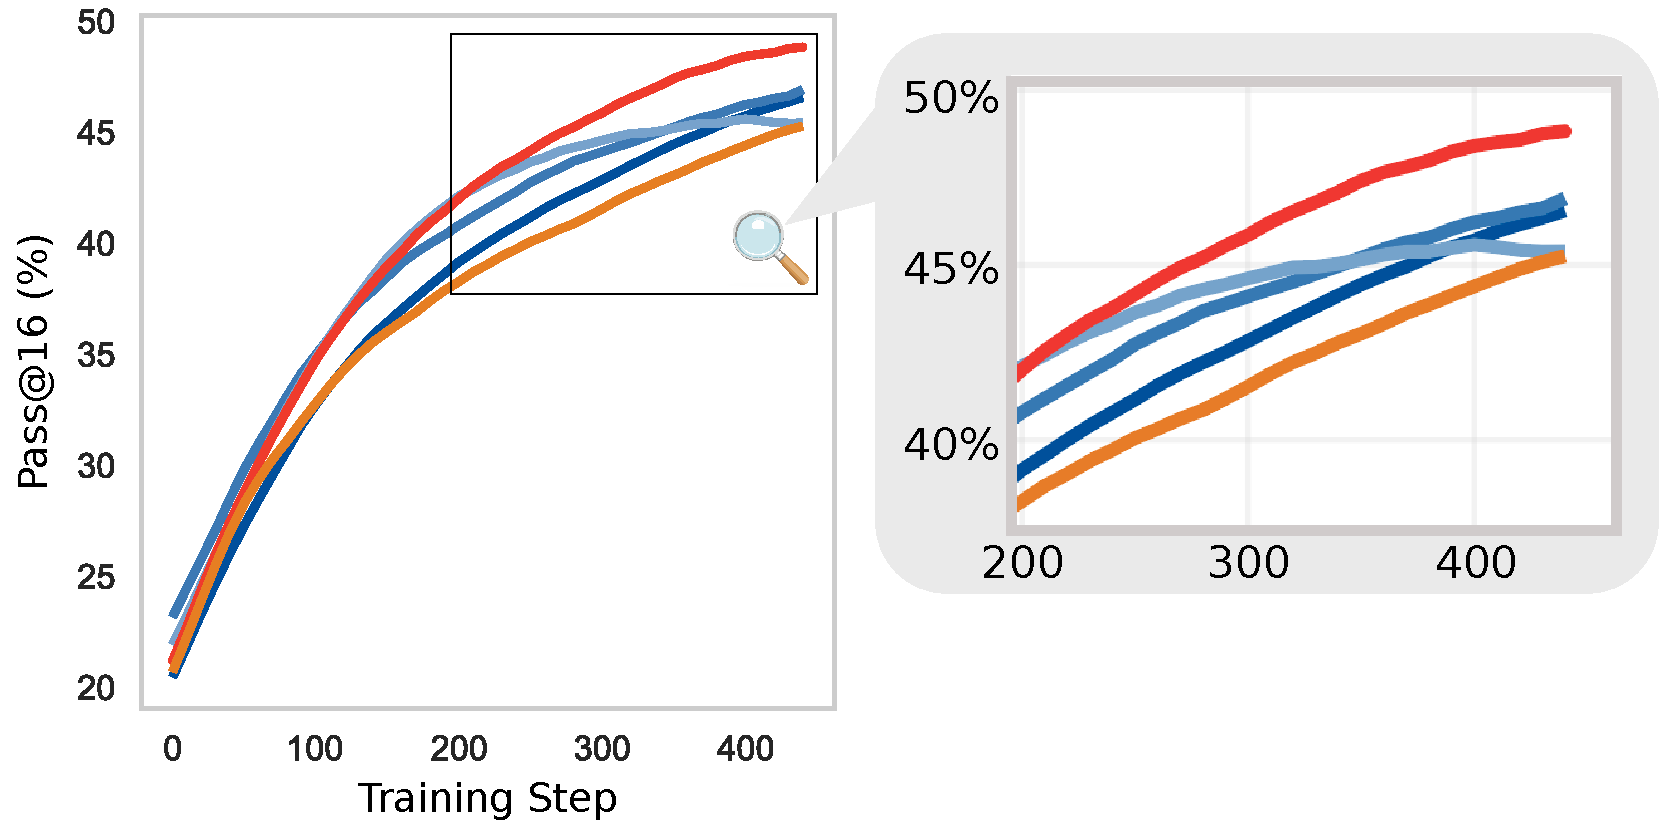
\includegraphics[width=\linewidth]{iclr2026/figures/best_at_16_Llama-3.2-1B-Instruct-new.pdf}
% \caption{Llama-3.2-1B-instruct}
% \end{subfigure}
% \begin{subfigure}[t]{0.44\textwidth}
% \centering
% 
\includegraphics[width=\linewidth]{iclr2026/figures/best_at_16_Qwen2.5-Math-1.5B-new.pdf}
% \caption{Qwen-2.5-Math-1.5B}
% \end{subfigure}
% \begin{subfigure}[t]{0.1\textwidth}
% \centering
% \vspace{-2.8cm}
% 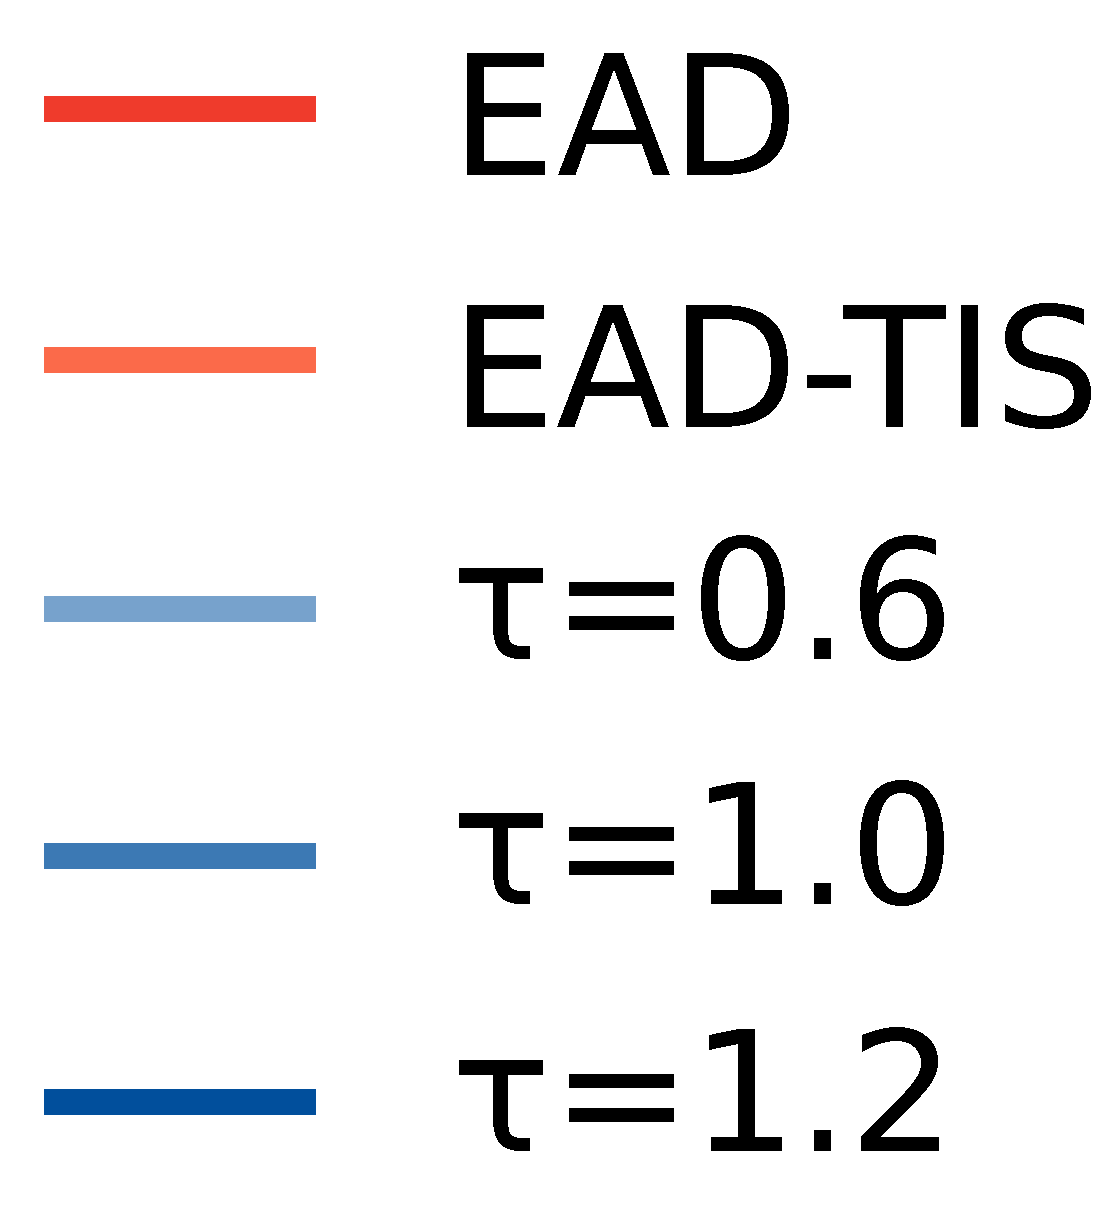
\includegraphics[width=\linewidth]{iclr2026/figures/legend-bon.pdf}
% \end{subfigure}
% \vspace{-0.1in}
% \caption{
% Pass@16 performance evaluation in RL training.
% %
% On Math-500, applying \alg to DAPO with both Llama-3.2-1B-Instruct and Qwen2.5-Math-1.5B significantly boosts performance.
% %
% % Pass@16 on Math-500 during RL training. 
% %
% % On both Llama-3.2-1B-Instruct and Qwen2.5-Math-1.5B, \alg enhances DAPO  
% % RL algorithm\zz{should we just say DAPO instead of RL algorithm?} over time, yielding significant gains in both performance and sample efficiency. 
% % \ych{Make it Figure 1! "sequential cool decoding"? (suggested by victor)}
% }
% \label{fig: main_bench_best_at_16}
% \vspace{-0.2in}
% \end{figure}
%
\begin{figure}[t!]
\centering
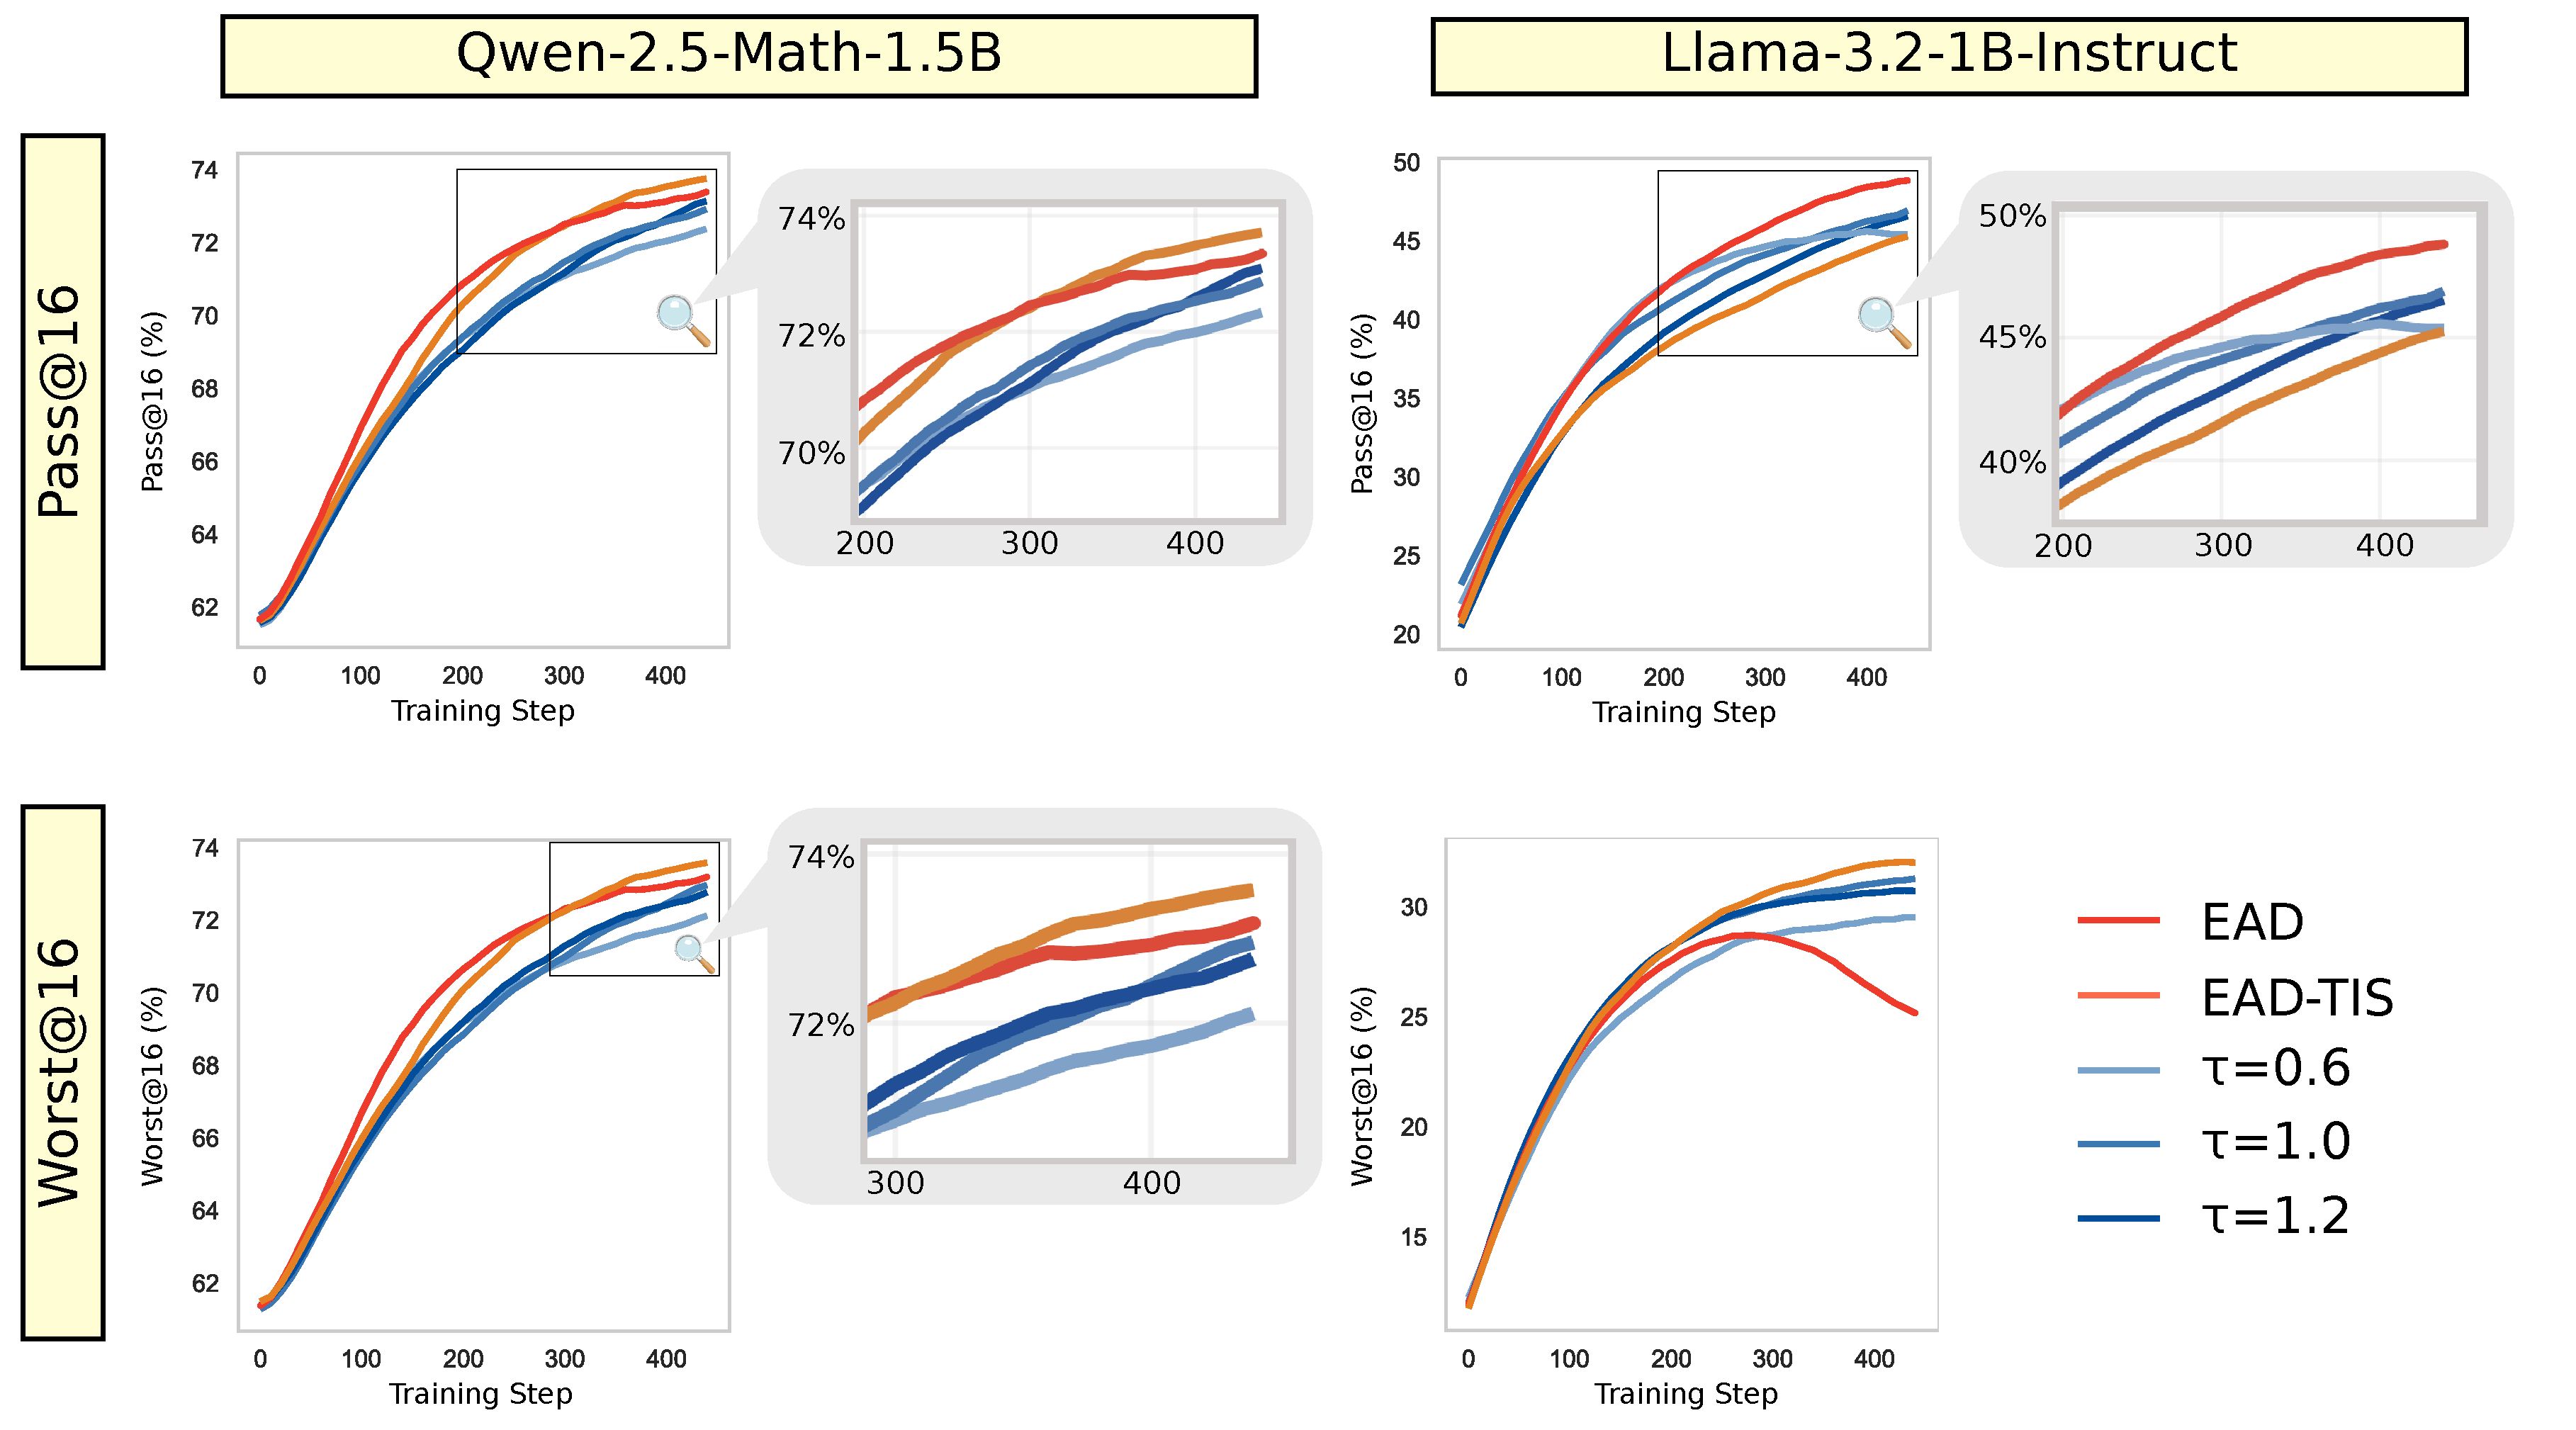
\includegraphics[width=\linewidth]{iclr2026/figures/best-and-worst-at-16.pdf}
% \vspace{-0.25in}
\caption{
Pass@16 and Worst@16 performance evaluation in RL training. 
%
% While in most of time, \alg can help model to explore high-quality samples in training for the whole distribution (so even the worst samples could win over samples from temperature sampling), this gain is not sustained, and importance sampling could step in as a good supplement to correct the bias and support prolonged training.  
%
While \alg improves exploration of high-quality samples (even the worst outperform temperature sampling), the gain diminishes over time; importance sampling can supplement to correct bias and sustain training.
}
\label{fig: main_bench_best_worst_at_16}
% \vspace{-0.2in}
\end{figure}
%
\begin{wrapfigure}{r}{0.45\textwidth}
\vspace{-0.15in}
    \centering
    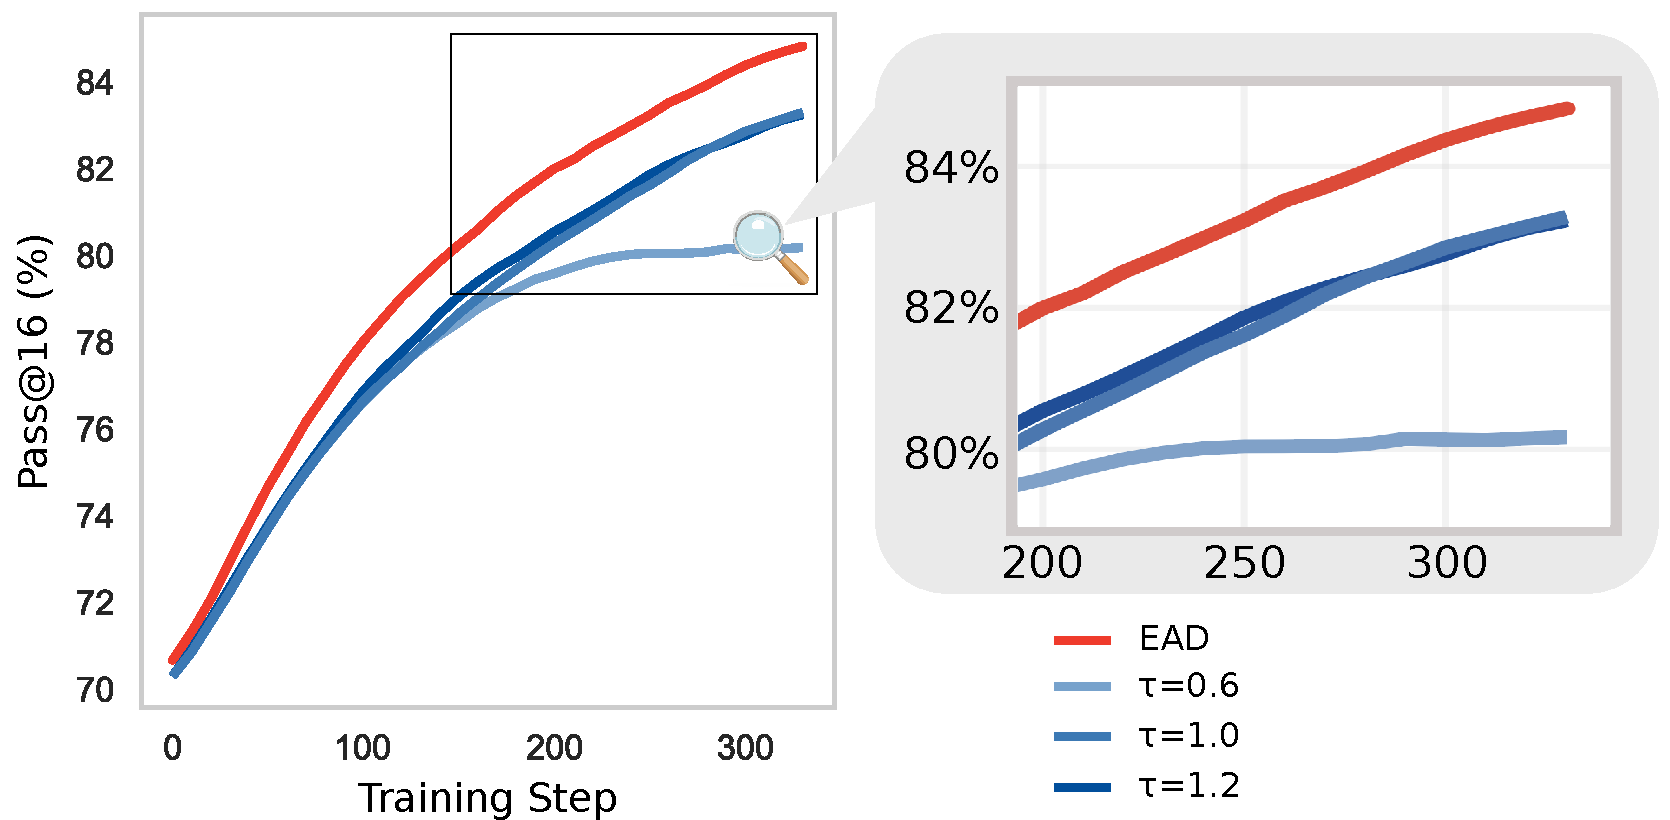
\includegraphics[width=\linewidth]{iclr2026/figures/best_at_16_Qwen2.5-Math-7B-new.pdf}
    \vspace{-0.2in}
    \caption{
    % Qwen-2.5-7B
    Pass@16 performance on Qwen-2.5-Math-7B. 
    %
    \alg enables better exploration than fixed-temperature sampling, yielding sustained gains in Pass@16 throughout training.
    %
    }
    % \vspace{-0.2in}
    \label{fig: best_at_16_qwen2.5_7b}
\end{wrapfigure}
%
As shown in \cref{fig: main_bench_best_worst_at_16}, \alg significantly improves training efficiency. 
%
For Pass@16 accuracy, 
% both \alg (w/o TIS) and \alg (w/ TIS) 
\alg (w/o TIS) consistently outperforms the baselines on the Llama and Qwen models (\alg (w/ TIS) also outperforms on the Llama model), demonstrating more effective exploration. 
%
Under the stricter Worst@16 metric, the inclusion of TIS becomes essential for maintaining stable performance gains, highlighting its importance for correcting the off-policy training dynamic introduced by \alg. 
%
Through bootstrapping evaluation as in~\citet{hochlehnert2025sober}, the standard deviation of both Pass@16 performance and worst@16 are way below 0.01 and thus all comparisons here are significant.
% \zz{is there a figure or table to support this sentence?}
%


%
% We further verify the experiment results with a larger model, Qwen2.5-Math-7B~\citep{yang2024qwen2}, and we demonstrate the experiment results in \cref{fig: best_at_16_qwen2.5_7b}. 

%
% We can see that the performance gain brought by \alg still significant when the model size is enlarged, verifying the generalization of our proposed method. 


To verify that our method generalizes, we evaluated it on the larger Qwen-2.5-Math-7B model. The results, presented in \cref{fig: best_at_16_qwen2.5_7b}, confirm that the performance gains from \alg remain significant. This demonstrates that our approach is effective not only on smaller models but also scales successfully.
%

% \begin{figure}[h!]
% \centering
% \begin{subfigure}[b]{0.44\textwidth}
%     \centering
%     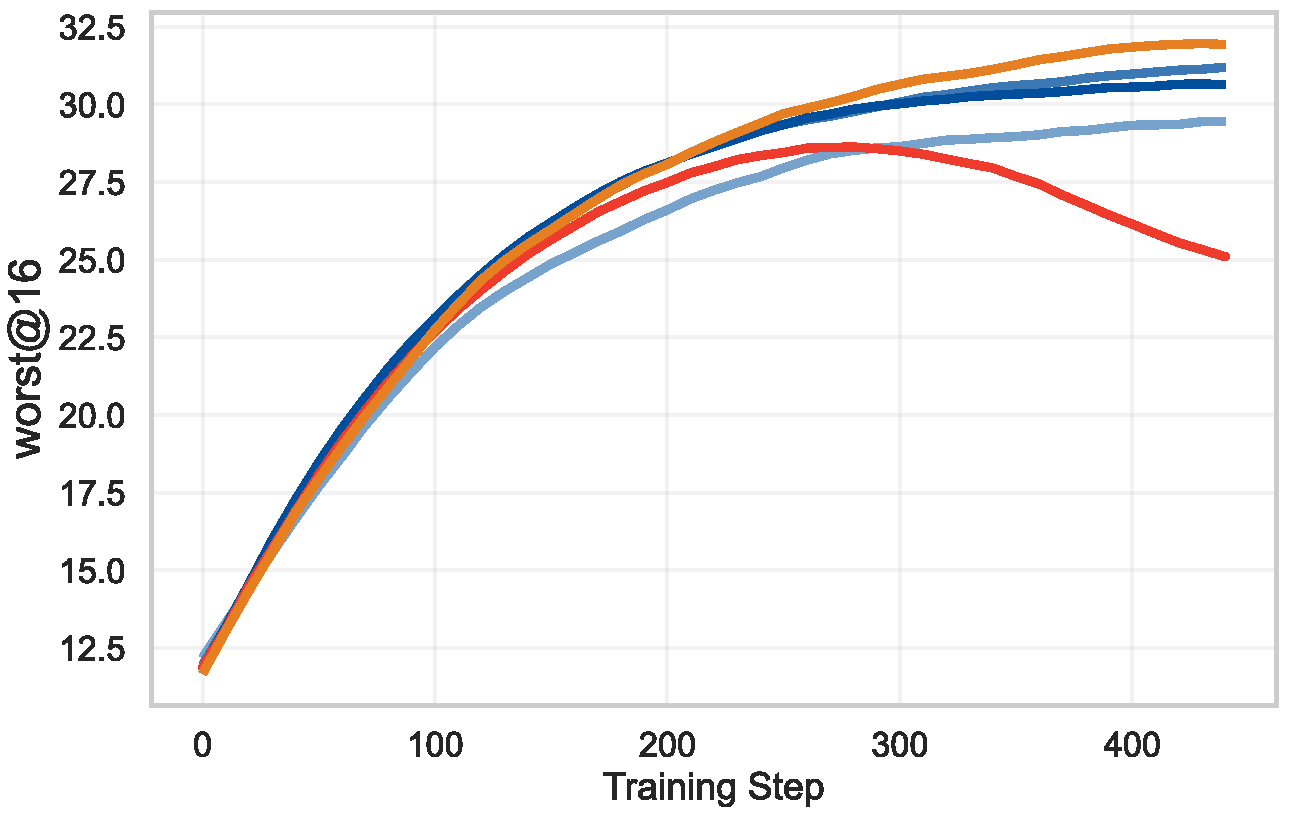
\includegraphics[width=\linewidth]{iclr2026/figures/worst_at_16_Llama-3.2-1B-Instruct.pdf}
%     \caption{Llama-3.2-1B-Instruct}
% \end{subfigure}
% \begin{subfigure}[b]{0.44\textwidth}
%     \centering
%     
\includegraphics[width=\linewidth]{iclr2026/figures/worst_at_16_Qwen2.5-Math-1.5B.pdf}
%     \caption{Qwen2.5-Math-1.5B}
% \end{subfigure}
% \begin{subfigure}[t]{0.1\textwidth}
%     \centering
%     \vspace{-3.5cm}
%     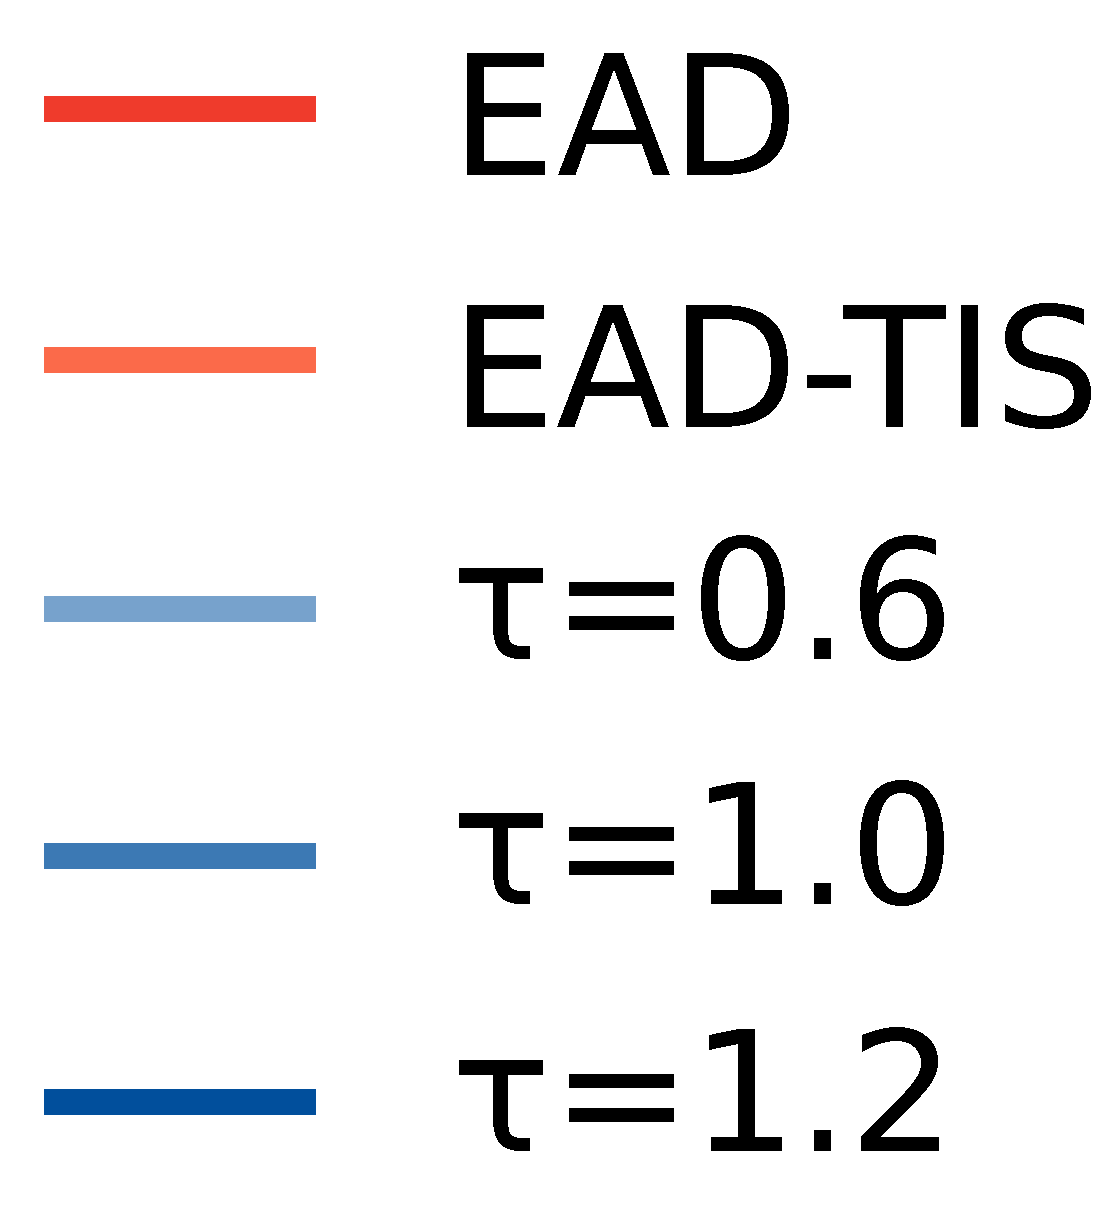
\includegraphics[width=\linewidth]{iclr2026/figures/legend-bon.pdf}
% \end{subfigure}
%   \caption{Worst@16 Performance Evaluation in RL Training. While in most of time, EAD could help model to explore high-quality samples in training for the whole distribution (so even the worst samples could win over ordinary multinomial samples), this gain is not sustained, and importance sampling could step in as a good supplement to correct the bias and support prolonged training.  }
%   \label{fig: main_bench_worst_at_16}
% \end{figure}

\begin{figure}[t]
% \begin{wrapfigure}{r}{0.6\textwidth}
    \centering
    \vspace{-0.05in}
    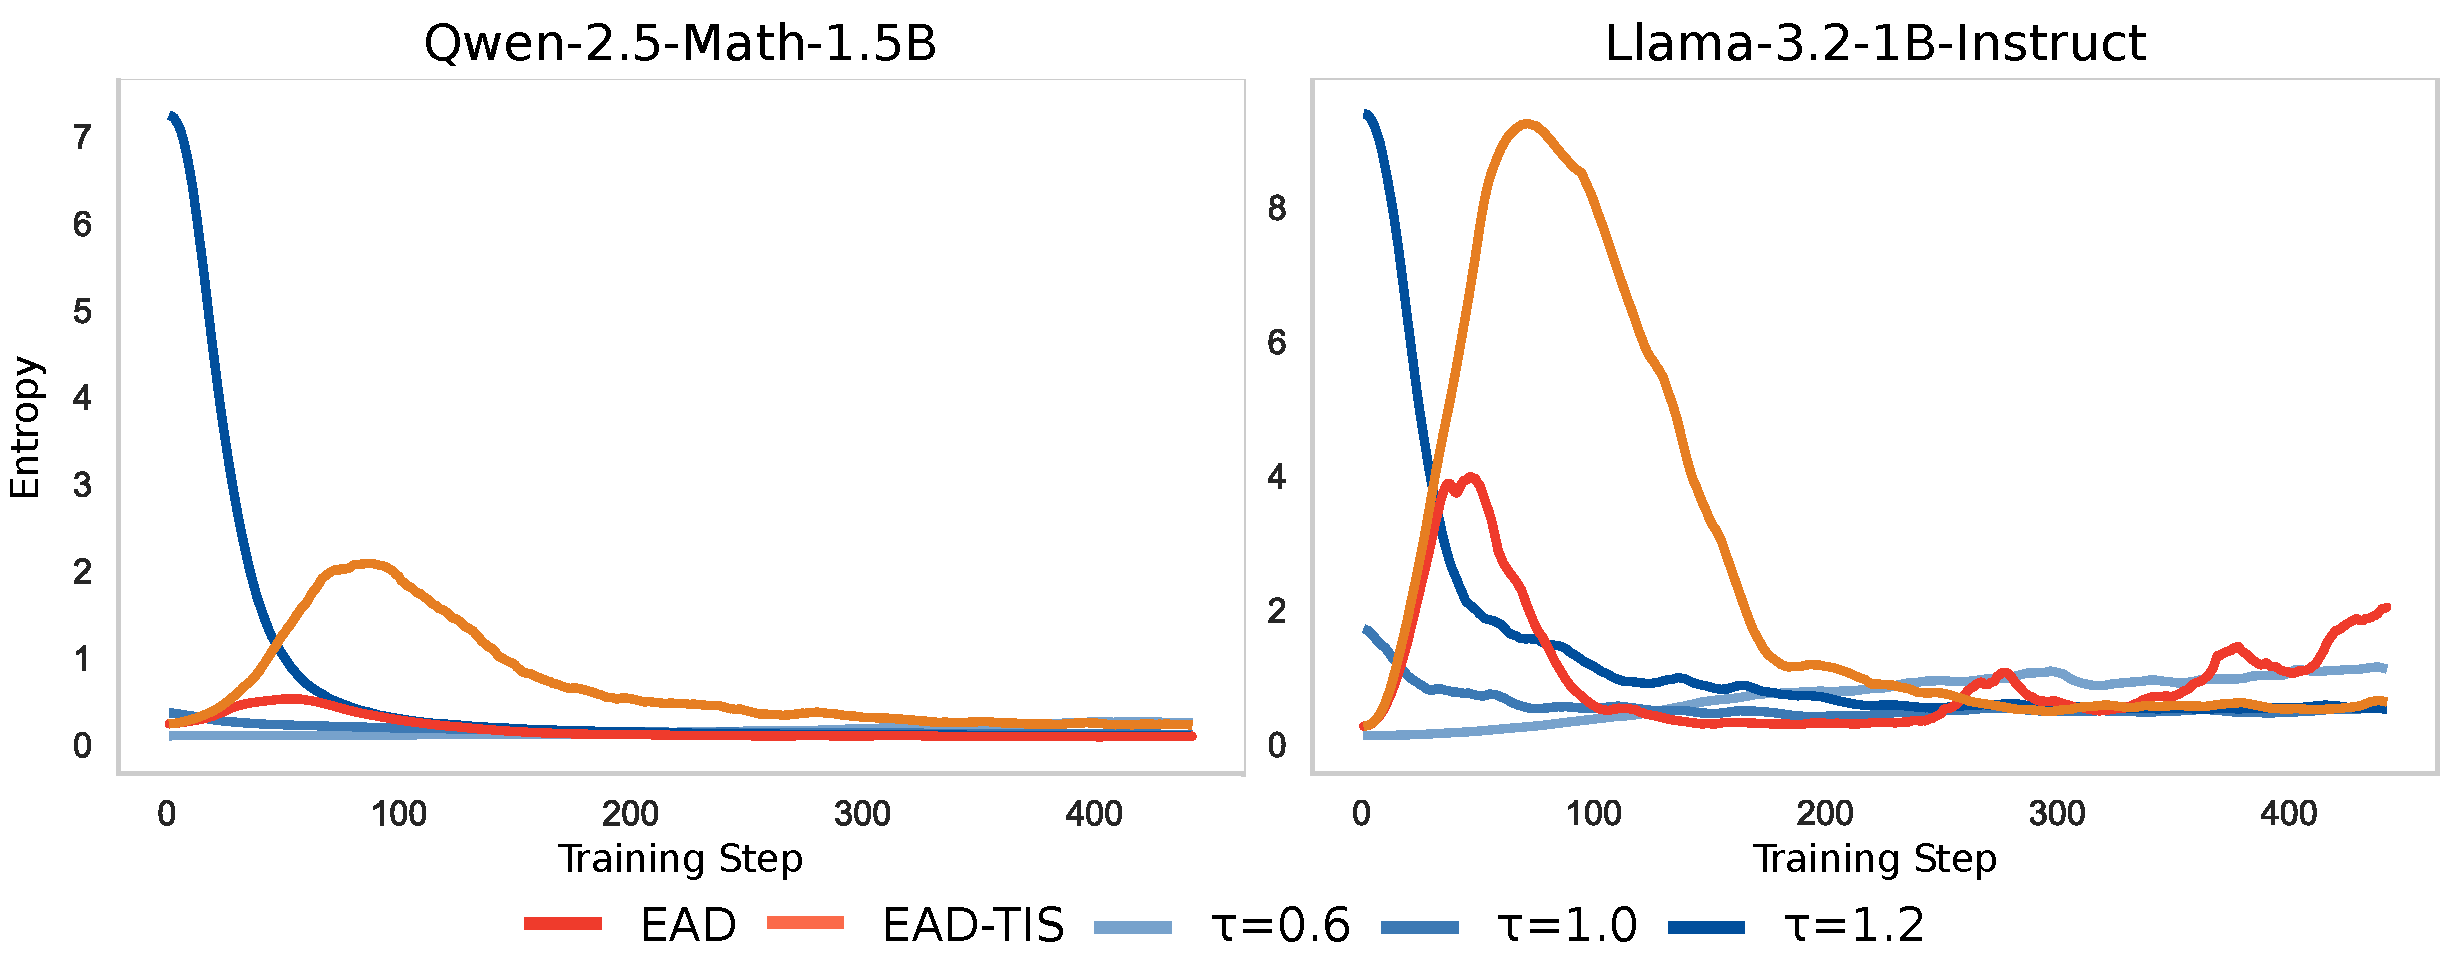
\includegraphics[width=.9\linewidth]{iclr2026/figures/entropy.pdf}
    \vspace{-0.1in}
    \caption{Entropy Dynamics in RL Training. Under commonly-used temperature sampling, trained with RL algorithm would make entropy decrease, sharply shrinking the exploration space for RL from beginning. While EAD could help RL algorithm to escape local minimum and do exploration when needed in the middle of RL training. 
    % \zz{Can we make the legend horizontal for this figure?}
    }
\label{fig: main_bench_entropy}
\vspace{-0.25in}
\end{figure}
% \end{wrapfigure}
%


\paragraph{\alg Mitigates Entropy Collapse.}
% One notorious problem in RLVR training is the entropy collapse problem~\citep{cui2025entropy}, which indicates the shrinkage of exploration space and limits the potential for the model to further improve at the later stage of RL training (``plateau stage''~\citep{dengres2025trial}). 
%
One major problem in RLVR training is entropy collapse~\citep{cui2025entropy}, which causes the exploration space to shrink and constrains improvement during the ``plateau stage"~\citep{deng2025trial}.
%
We plot the entropy dynamic in \cref{fig: main_bench_entropy}, where we can see that the entropy dynamic for \alg-empowered methods is not monotonically decreasing from the beginning. 
%
Instead, it tries to gradually transition out from local optimum~\citep{kirkpatrick1983optimization, bertsimas1993simulated} in a natural, continuous way without any external intervention, such as introducing tree search in rollout sampling~\citep{li2025treepo}.
%
\begin{wrapfigure}{r}{0.6\textwidth}
% \begin{figure}[t]
\begin{subfigure}{\linewidth}
    \centering
    \vspace{-0.1in}
    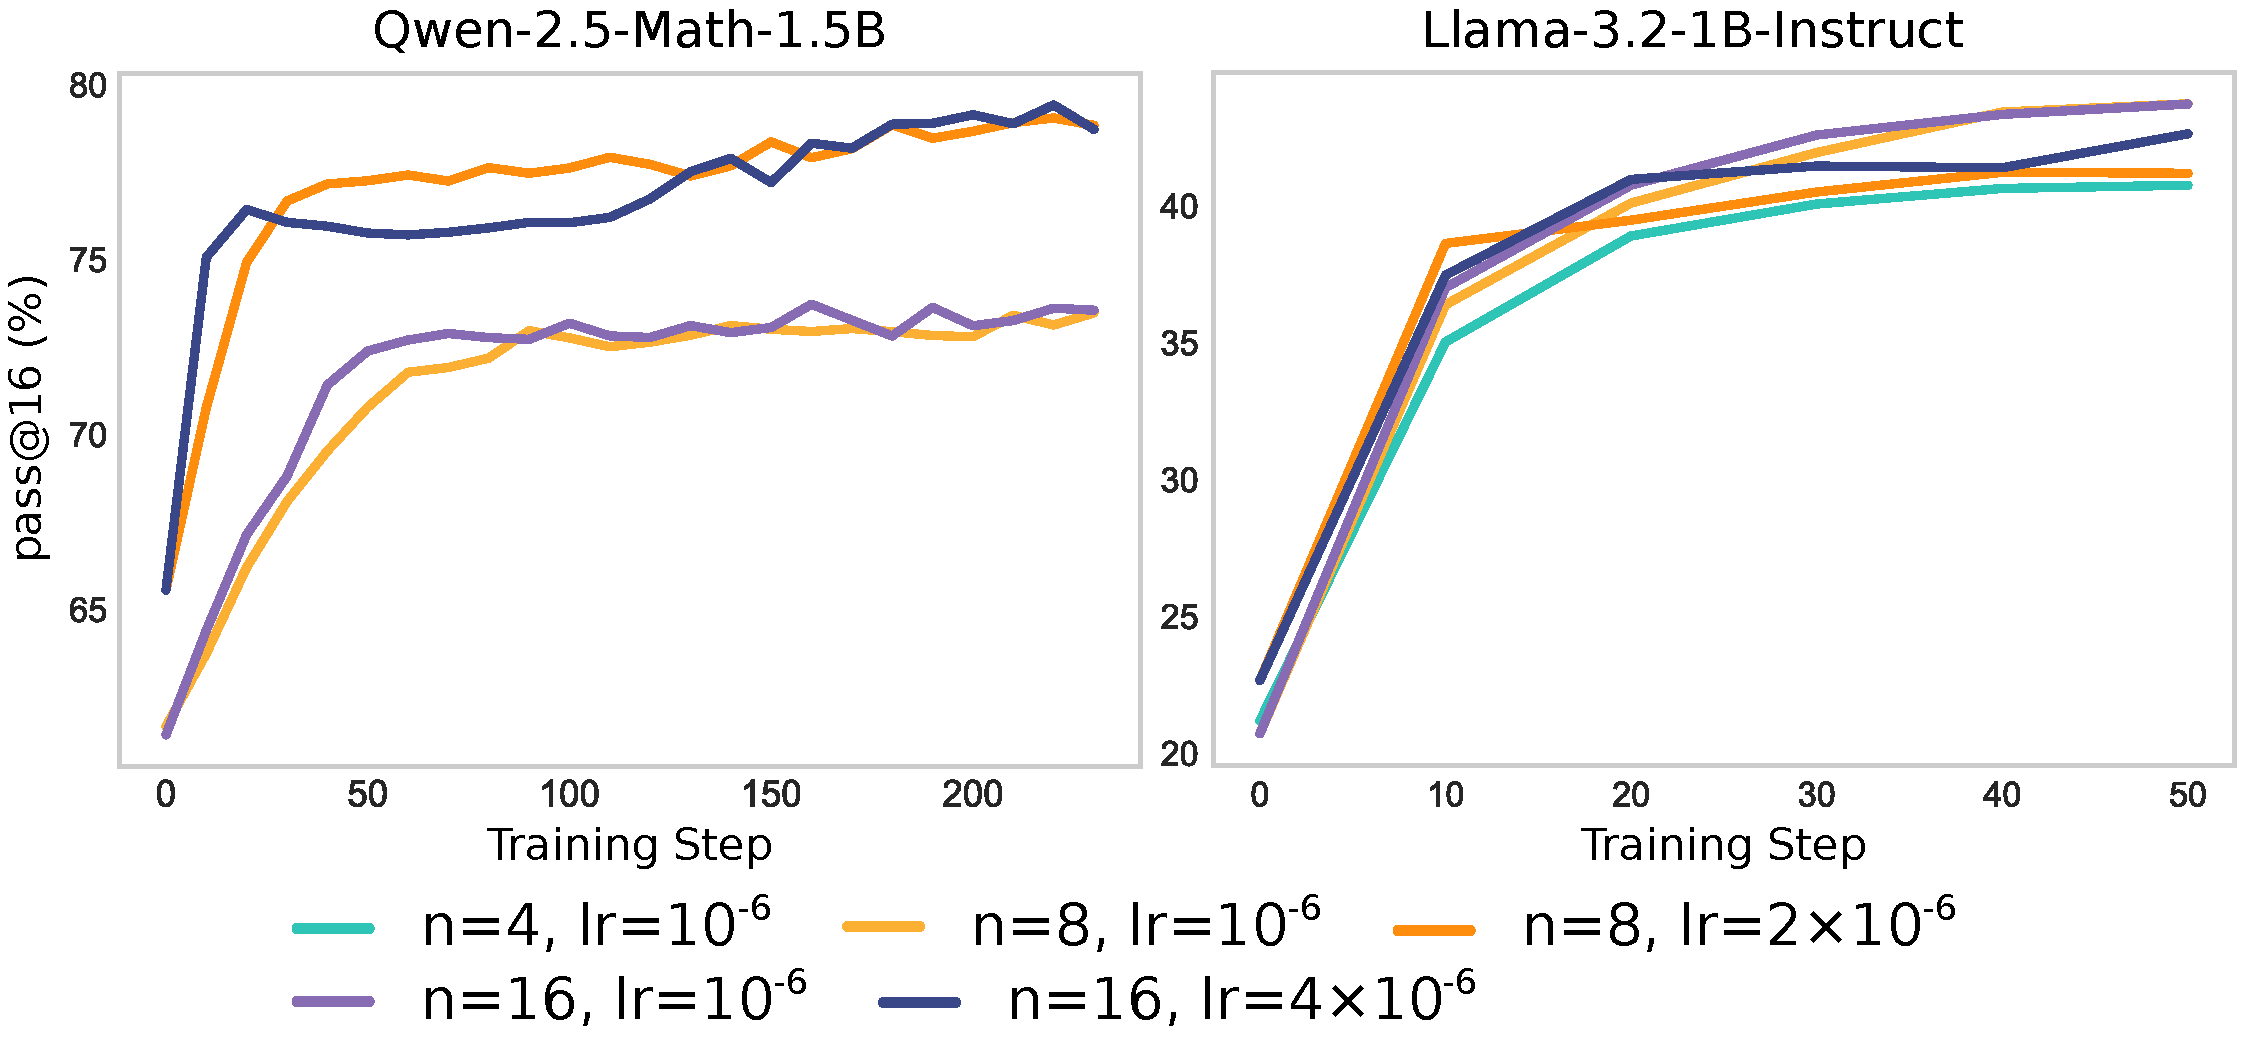
\includegraphics[width=\linewidth]{iclr2026/figures/scaling_rollout/scaling-rollout.pdf}
    \vspace{-0.15in}
    \caption{\alg would bring further performance improvement via increased numbers of rollouts, but the commonly used $4$ or $8$ is already good enough. }
    \label{fig: main_bench_rollout_scaling}
% \vspace{-0.4in}
\end{subfigure}
% \end{figure}
\begin{subfigure}{\linewidth}
% \begin{figure}[h!]
    % \vspace{-0.4in}
    \centering
    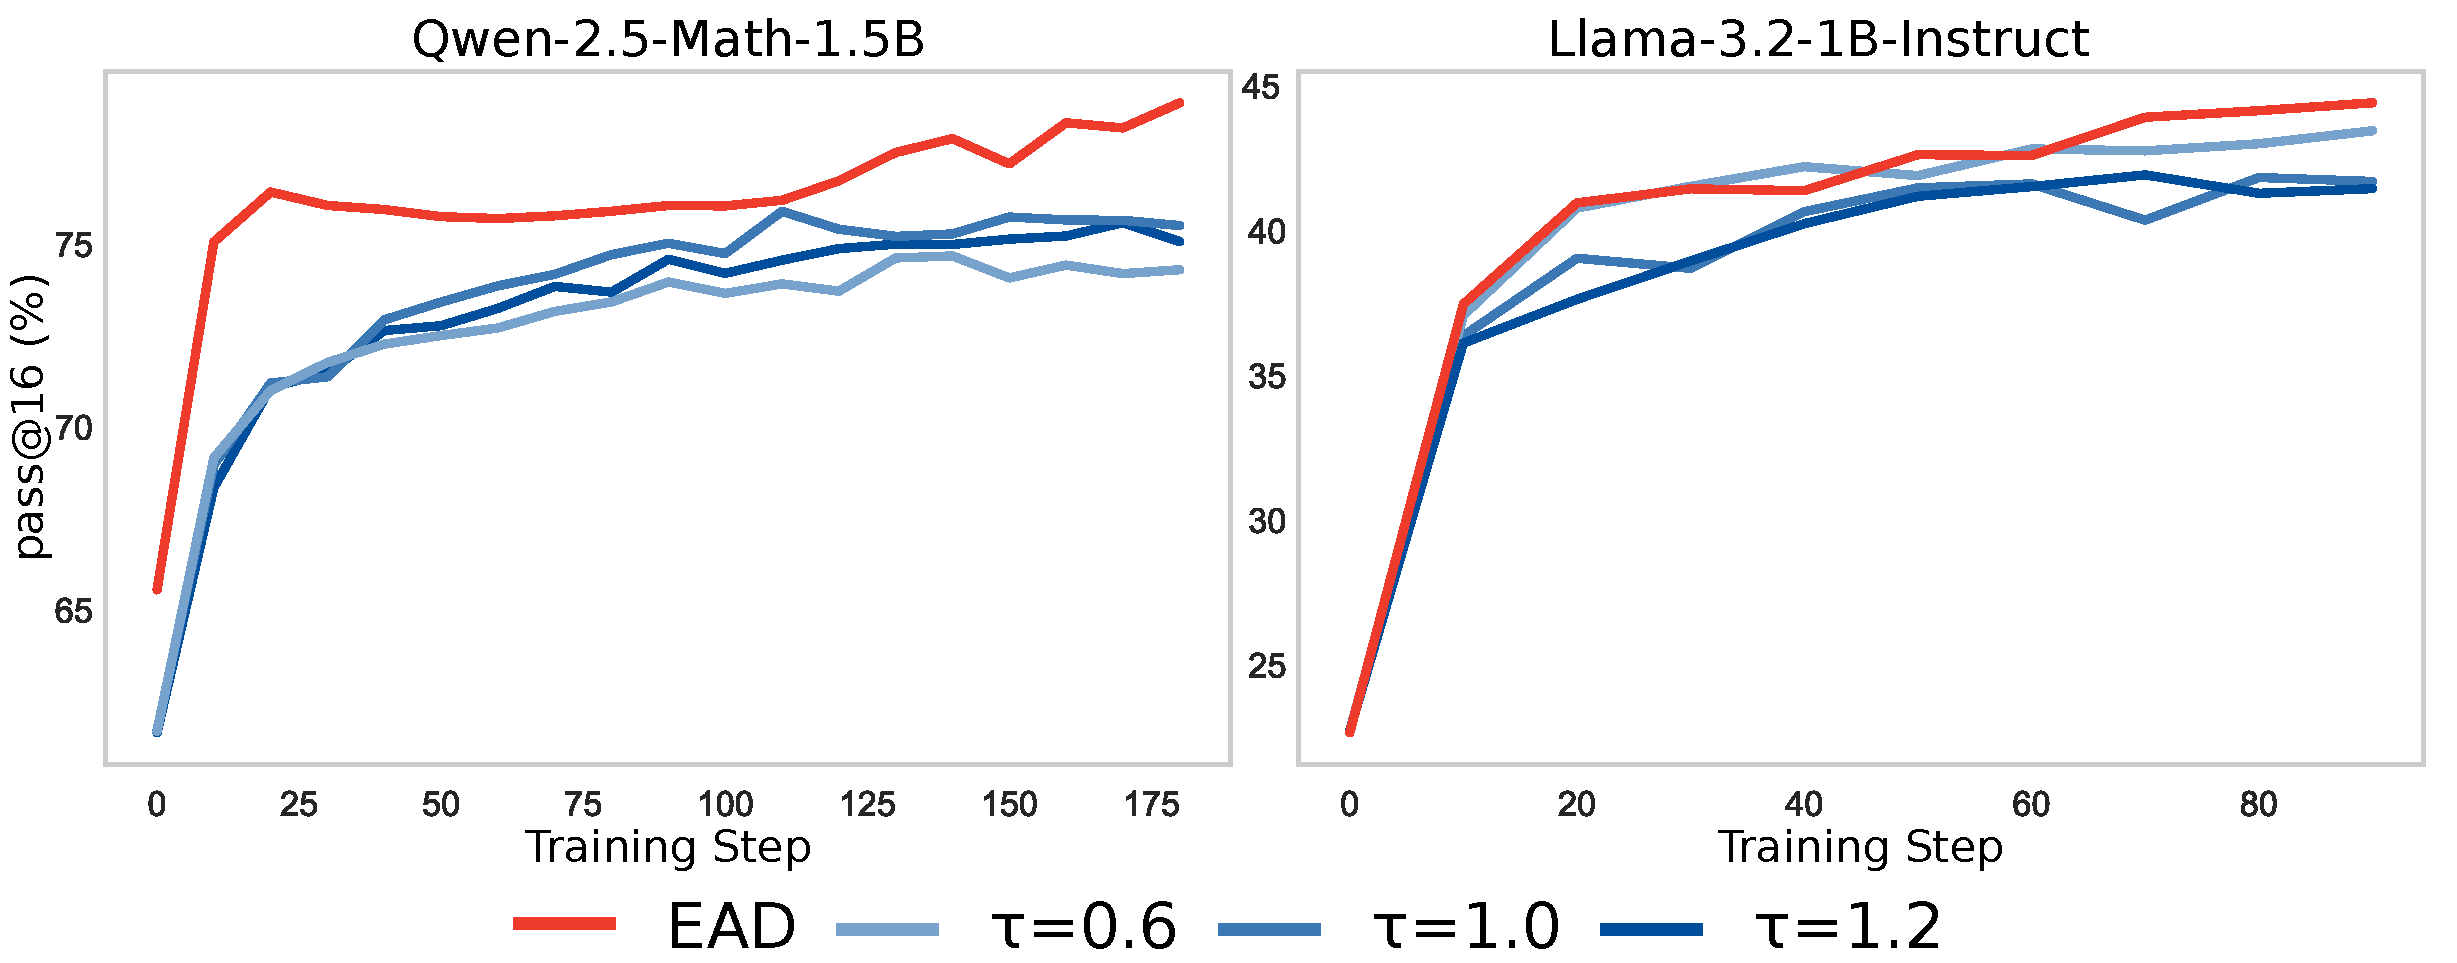
\includegraphics[width=\linewidth]{iclr2026/figures/rollout16_modelwise_compare/rollout-16.pdf}
    % \vspace{-0.25in}
    \caption{When scaling out the rollout number to 16, the relative advantages of our methods diminished; however, it still outperforms traditional same-temperature sampling.}
    \label{fig: rollout_modelwise_compare}
    \vspace{-0.1in}
% \end{figure}
\end{subfigure}
\caption{Sample Efficiency of EAD. }
\vspace{-0.3in}
\end{wrapfigure}
%

%


% \paragraph{Sample Efficiency of \algname.}
% While expensive, upsampling rollouts ~\citep{hou2025t1} is a common strategy to encourage exploration in RL training and is orthogonal to our \algname strategy. We demonstrate the rollout scaling results in \cref{fig: main_bench_rollout_scaling}. We also vary the learning rate following the empirical observation in \citep{chen2025pass} that rollout upsampling will be more effective with larger learning rate. Here we can find that upsampling rollouts would also help EAD improve the performance, but the commonly used $4$ or $8$ rollout is already good enough for RL training ($n=8$, learning rate$=10^{-6}$ works best for Llama-3.2-1B-Instruct, $n=8$, learning rate$=2\times10^{-6}$ works best for Qwen2.5-Math-1.5B). This indicates great sample efficiency of Annealed Sampling and help save the computation in rollout sampling. 


\paragraph{Sample efficiency of \alg.}
Increasing the number of rollouts is a common but computationally expensive strategy to enhance exploration~\citep{hou2025t1}. 
%
We test the sample efficiency of \alg by varying the number of rollouts, adjusting the learning rate accordingly as suggested by prior work~\citep{chen2025pass}. 
%
As shown in \cref{fig: main_bench_rollout_scaling}, while more rollouts can further improve performance, \alg achieves strong results with just 4 or 8 rollouts. 
%
For instance, the optimal configurations are $n=8$ with a learning rate of $10^{-6}$ for Llama-3.2-1B-Instruct and $2\times10^{-6}$ for Qwen-2.5-Math-1.5B. 
%
This highlights the sample efficiency of our approach, offering a way to reduce the computational cost of the rollout phase.
%

To assess whether \alg's advantage persists with extensive exploration, we compare it against baselines using a larger set of 16 rollouts. 
%
\cref{fig: rollout_modelwise_compare} shows that although the relative performance gain diminishes, \alg still outperforms fixed-temperature baselines by a clear margin.
%


% We further compare with our baseline on extended $16$ rollouts to assess whether the advantage brought by our method would fade away with sufficient rollouts. The results are demonstrated in \cref{fig: rollout_modelwise_compare}. We see that though the relative edge of our method over traditional temperature sampling shrinks, our method still outperforms traditional temperature sampling by a clear margin. 



%


% \subsection{\algname works with various RL algorithms}
% To demonstrate that \alg can plug-and-play with various RL algorithms as a better exploration method than normal temperature sampling, we additionally verify the effectiveness of \alg in GRPO~\citep{shao2024deepseekmath} and EntropyMech~\citep{cui2025entropy}. Compared to more exploration-promoting DAPO, GRPO adds a KL divergence term to the reference model $\pi_{\text{ref}}$ and enforces a stricter limitation on probability changes, which could hurt the exploration~\citep{yu2025dapo}. EntropyMech adopts a more complicated log-probability-advantage covariance to clip tokens, mitigating entropy collapse. 

% We demonstrate our results compared with baselines in \cref{fig: algorithm_wide_comparison}, where we can see \alg performs better than temperature sampling, demonstrating its wide applicability. 


\subsection{\alg is Compatible with Various RL Algorithms}
\begin{wrapfigure}{r}{.5\linewidth}
    \centering
    % \vspace{-0.5in}
    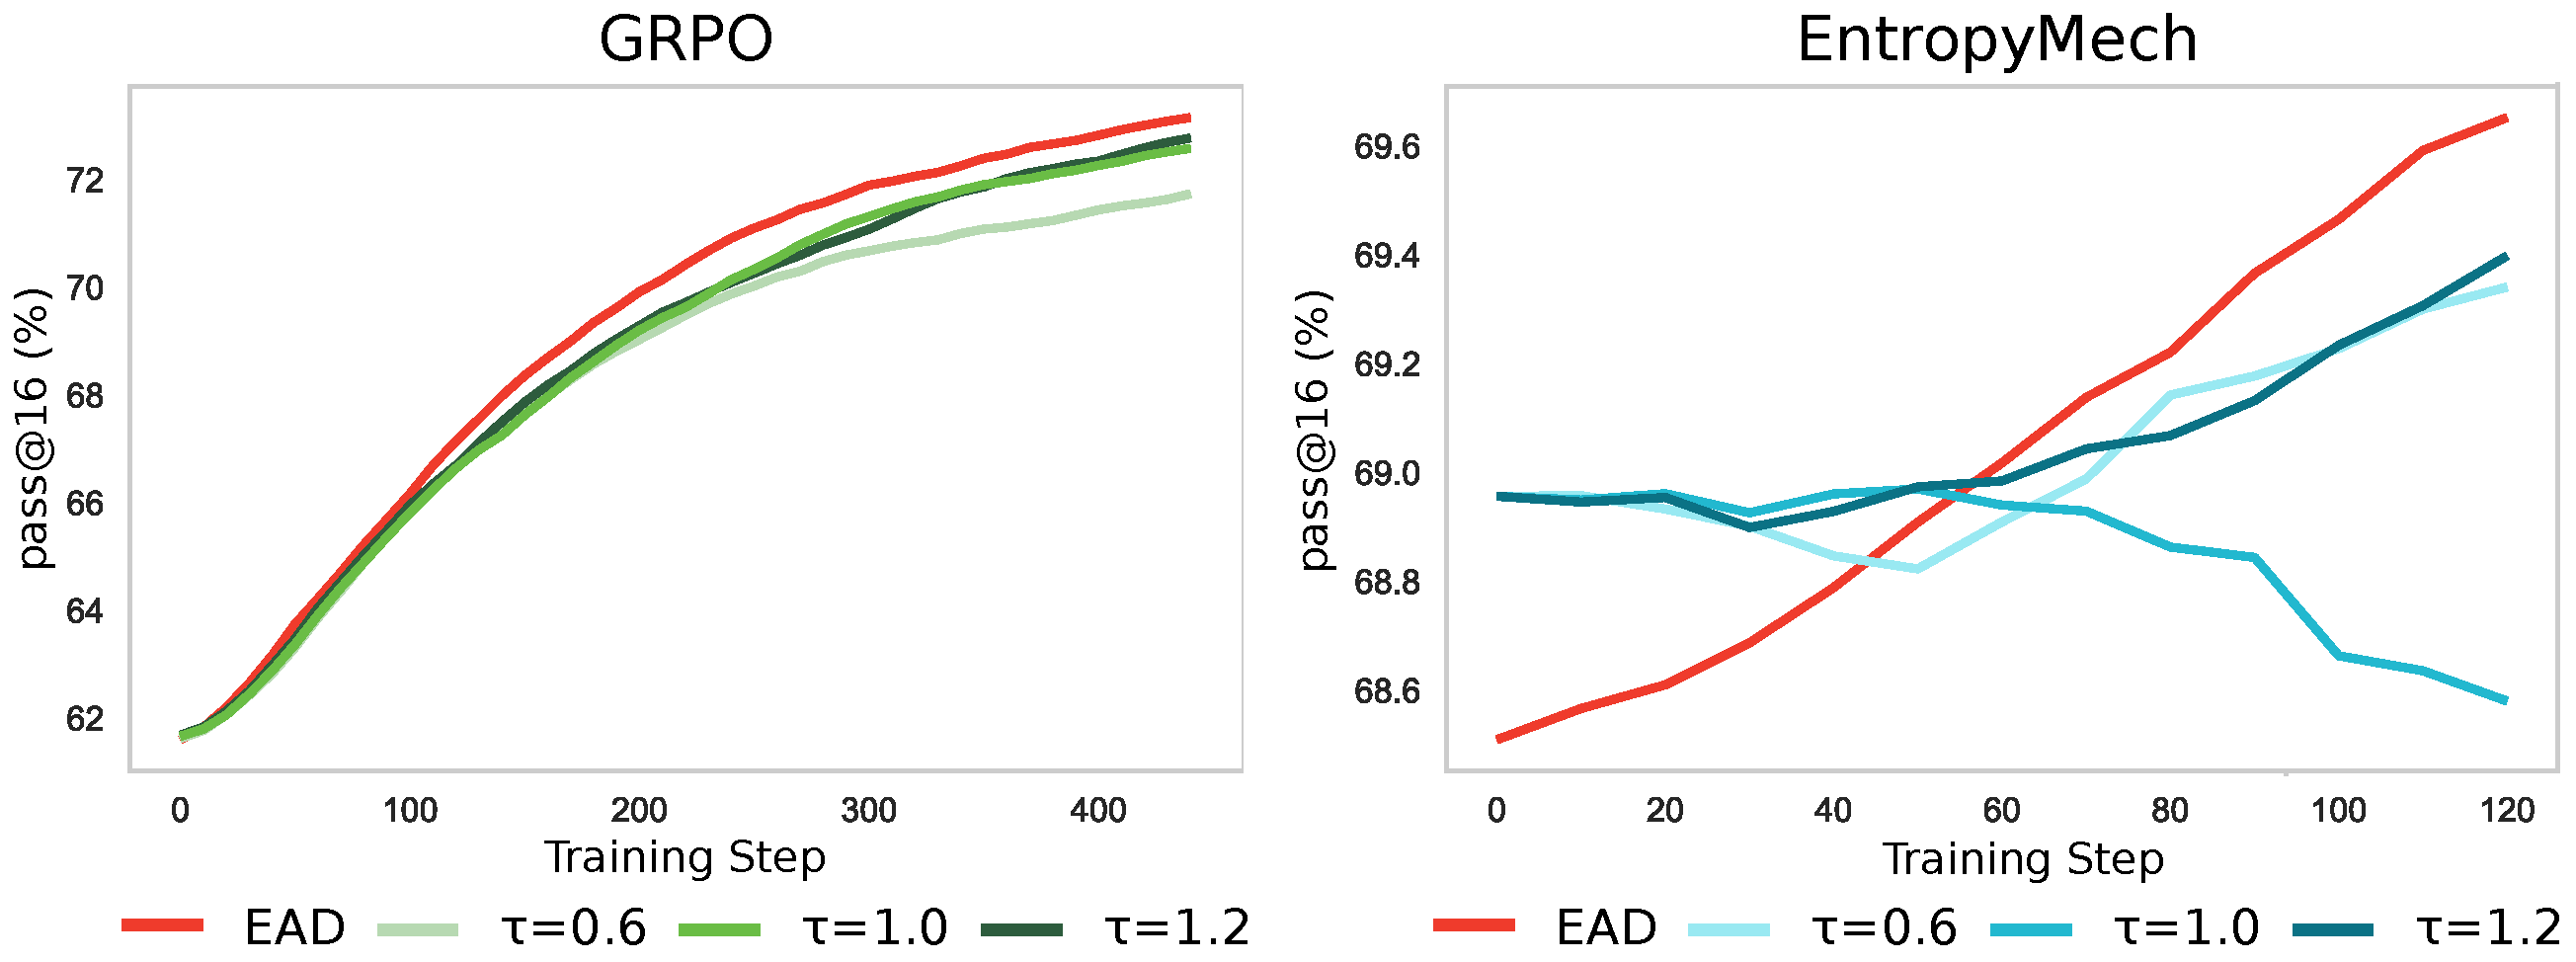
\includegraphics[width=\linewidth]{iclr2026/figures/diff-method.pdf}
    \vspace{-0.1in}
    \caption{\alg is compatible with various RL algorithms and can significantly improve the model performance over time. } 
    \label{fig: algorithm_wide_comparison}
    \vspace{-0.2in}
    \end{wrapfigure}
% \vspace{-0.1in}
To demonstrate that \alg is a general, plug-and-play exploration strategy, we evaluate its performance when integrated into two other prominent RL algorithms: GRPO~\citep{shao2024deepseekmath} and EntropyMech~\citep{cui2025entropy}. 
%
These algorithms provide diverse testbeds. 
%
GRPO is more conservative, constraining policy updates with a KL divergence penalty and stricter clipping mechanism that can limit exploration~\citep{yu2025dapo}, while EntropyMech uses a specialized token-clipping mechanism to mitigate entropy collapse. 
%

% \begin{figure}[t]
% % \begin{figure}[h!]
% % \vspace{-0.17in}
%     \centering
    
% % \end{figure}
% % \vspace{-0.3in}
% % \end{figure}
% % \begin{figure}[t]
% \hspace{0.1in}

% \end{figure}

%
As shown in \cref{fig: algorithm_wide_comparison}, \alg consistently outperforms fixed-temperature sampling in both frameworks. 
%
These results confirm the broad applicability of our method as an improved exploration strategy across different RL algorithms.

\subsection{\alg Improves Inference-Time Scaling}
\begin{wrapfigure}{r}{.45\linewidth}
    \centering
    \vspace{-0.7in}
    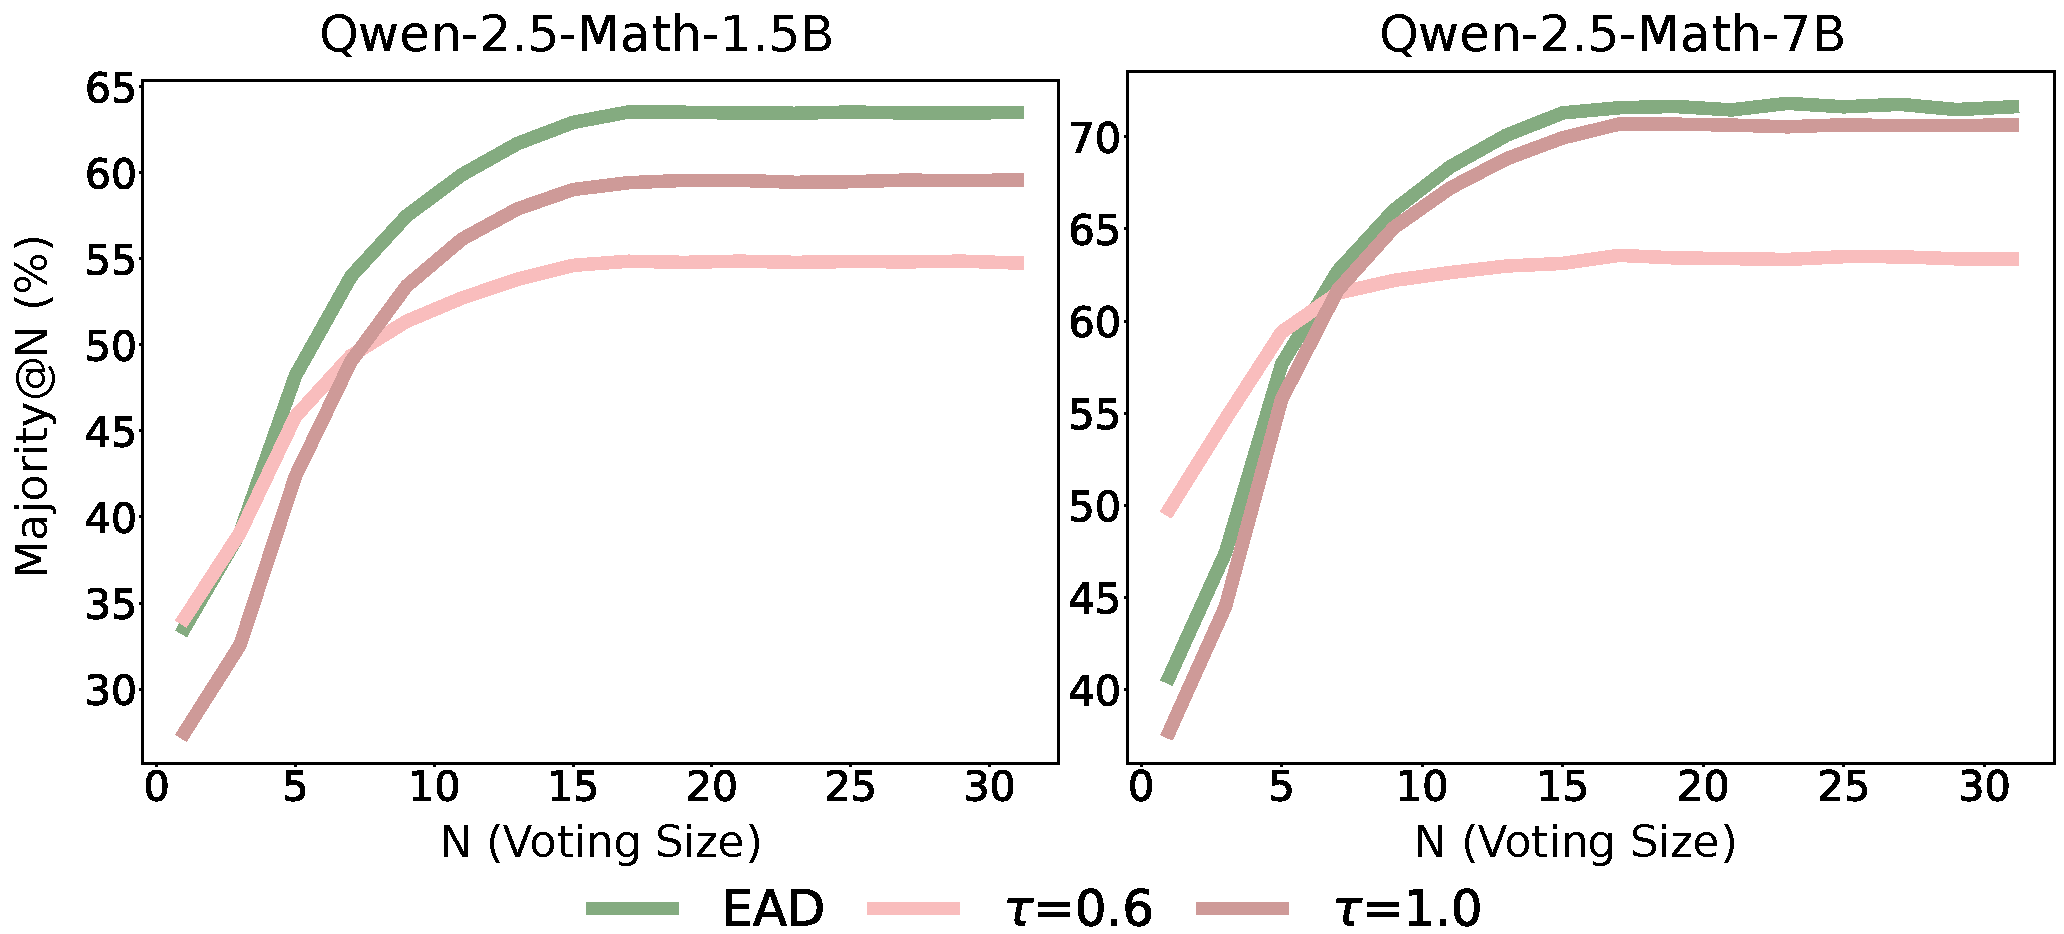
\includegraphics[width=\linewidth]{iclr2026/figures/inference_time_scaling/test-time.pdf}
    % \vspace{-0.25in}
    \caption{Inference-Time Scaling Evaluation for Different Decoding Methods using off-the-shelf Qwen2.5 models. We could see that \alg improves traditional temperature sampling. We set $\tau_{\text{max}}=1.2, \tau_{\text{min}}=0.1, d=25$ for \alg. }
    \label{fig: inference_time_scaling}
    \vspace{-0.2in}
    \end{wrapfigure}
%
To understand whether the success of \alg in RL training is driven by its ability to generate high-quality samples, we conduct an evaluation at inference time. 
%
This experiment is designed to isolate the sampling strategy's effectiveness from the dynamics of RL optimization~\citep{berseth2025exploration}. 
%
Using off-the-shelf Qwen-2.5 models without any fine-tuning, we compare \alg against fixed-temperature sampling. 
%
We use majority voting ($\text{Majority}@N$) to measure how performance scales with the number of samples $N$~\citep{wang2023selfconsistency, snell2024scaling}. 
%
As shown in \cref{fig: inference_time_scaling}, \alg consistently improves over the baseline for most values of $N$. 
%
This result confirms that \alg's advantage stems from its inherent capacity to discover higher-quality solutions, even without any training.
%
% \revise{
% \subsection{Ablation Study}

% \paragraph{Reverse Annealing} A counter-intuitive baseline would be we increase the tempearture through the generation process, rather than decreasing it. We take a simple schedule: 
% $\tau_t = \min\{\tau_\mathrm{min} + e^{t/d}, \tau_\mathrm{max}\}$
% We demonstrate the performance of such reverse-annealing temperature schedule (``revEAD'') in \cref{fig: reverse_annealing}. Here we can see that reverse annealing does not work. 
% \begin{figure}[t]
%     \centering
%     
\includegraphics[width=.75\linewidth]{iclr2026/figures/reverse_annealing/best_at_16_Qwen2.5-Math-1.5B.pdf}
%     \vspace{-0.1in}
%     \caption{Reverse Annealing does not even beat normal temperature sampling, verifying the necessity of using an annealing temperature schedule.  } 
%     \label{fig: reverse_annealing}
    
% \end{figure}

% \paragraph{Hyperparameter Sensitivity} 
% We do ablation to examine the hyperparameter sensitivity for the cap $d_{\max}$ and $\alpha$ in the global-step-aware decay rate. As shown in \cref{fig: ablation_cap}, we can see that as long as $d_{\max}$ is large enough to assure a smooth temperature annealing schedule, \alg is robust to wide range selection for $d_{\max}$. For very small $d_0=d_{\max}=25$, essentially the schedule won't change along the training (setting the growth factor $\alpha=0$ would achieve the same result), we see the abrupt performance drop, potentially because it cannot adapt to the increasing response length in training accordingly, as we explain in \cref{app: increased_length}. Another way to smooth out the temperature annealing schedule is to use a large $d_0$, then even $\alpha=0$ (same schedule along the training), overall the training would still be stable, even though the performance under large $d_0$ would increase slowly as the overall sequential exploration has become conservative, as shown in \cref{fig: ablation_growth_factor_and_decay_freq_init}.

% \begin{figure}[t]
%     \centering
%     
\includegraphics[width=.75\linewidth]{iclr2026/figures/ablation_cap/best_at_16_Qwen2.5-Math-1.5B.pdf}
%     \vspace{-0.1in}
%     \caption{Ablation study on decay cap $d_{\max}$. ``\alg'' refers to original $d_{\max}=40,000$ setup. Note, when cap $d_{\max}=25$, as $d_0=25$, this is essentially working as the fixed temperature annealing schedule along the training, essentially equivalent to setting $\alpha=0$.  We can see \alg is robust enough to a wide range of the decay cap $d_{\max}$ (e.g, as long as $>=200$), as long as the temperature can be reduced smoothly and react appropriately to increasing response length. Otherwise, the performance could drop in mid of training.} 
%     \label{fig: ablation_cap}
%     \vspace{-0.2in}
% \end{figure}

% \begin{figure}[t]
%     \centering
%     
\includegraphics[width=.75\linewidth]{iclr2026/figures/ablation_growth_factor_and_decay_freq_init/best_at_16_Qwen2.5-Math-1.5B.pdf}
%     \vspace{-0.1in}
%     \caption{Ablation study on growth factor and $d_0$. For small $d_0$, we have to set the growth factor $\alpha > 0$ to react to increasing response length so the overall temperature annealing schedule intra-sequence would be smooth. When $d_0$ is large, the overall temperature annealing schedule is very smooth at the beginning, and even setting $\alpha=0$ won't affect the training performance. However, this neglects exploration and lead to worse learning efficiency.  } 
%     \label{fig: ablation_growth_factor_and_decay_freq_init}
%     \vspace{-0.2in}
% \end{figure}

% }

% \revise{
% \subsection{Stress Test: DAPO-16K Recipe for AIME24}
% To further verify the effectiveness of our \alg under most realistic math reasoning tasks, we stress-test \alg with community-recognized DAPO~\citep{yu2025dapo} recipe, where the training dataset is DAPO-16k and the test set is the challenging AIME 2024 benchmark. To fit in the GPU memory we have, we use a smaller Qwen-3-8B-Base~\citep{yang2025qwen3} model instead of 32B model and reduce the maximum response length from $20,480$ to $8,192$. We set $d_0=500, d_{\max}=40,000$ and vary $\alpha=5, 50$ for \alg. We can see that \alg successfully outperforms the common temperature sampling baseline and achieves significant learning efficiency in \cref{fig: aime24}. 

% \begin{figure}[t]
%     \centering
%     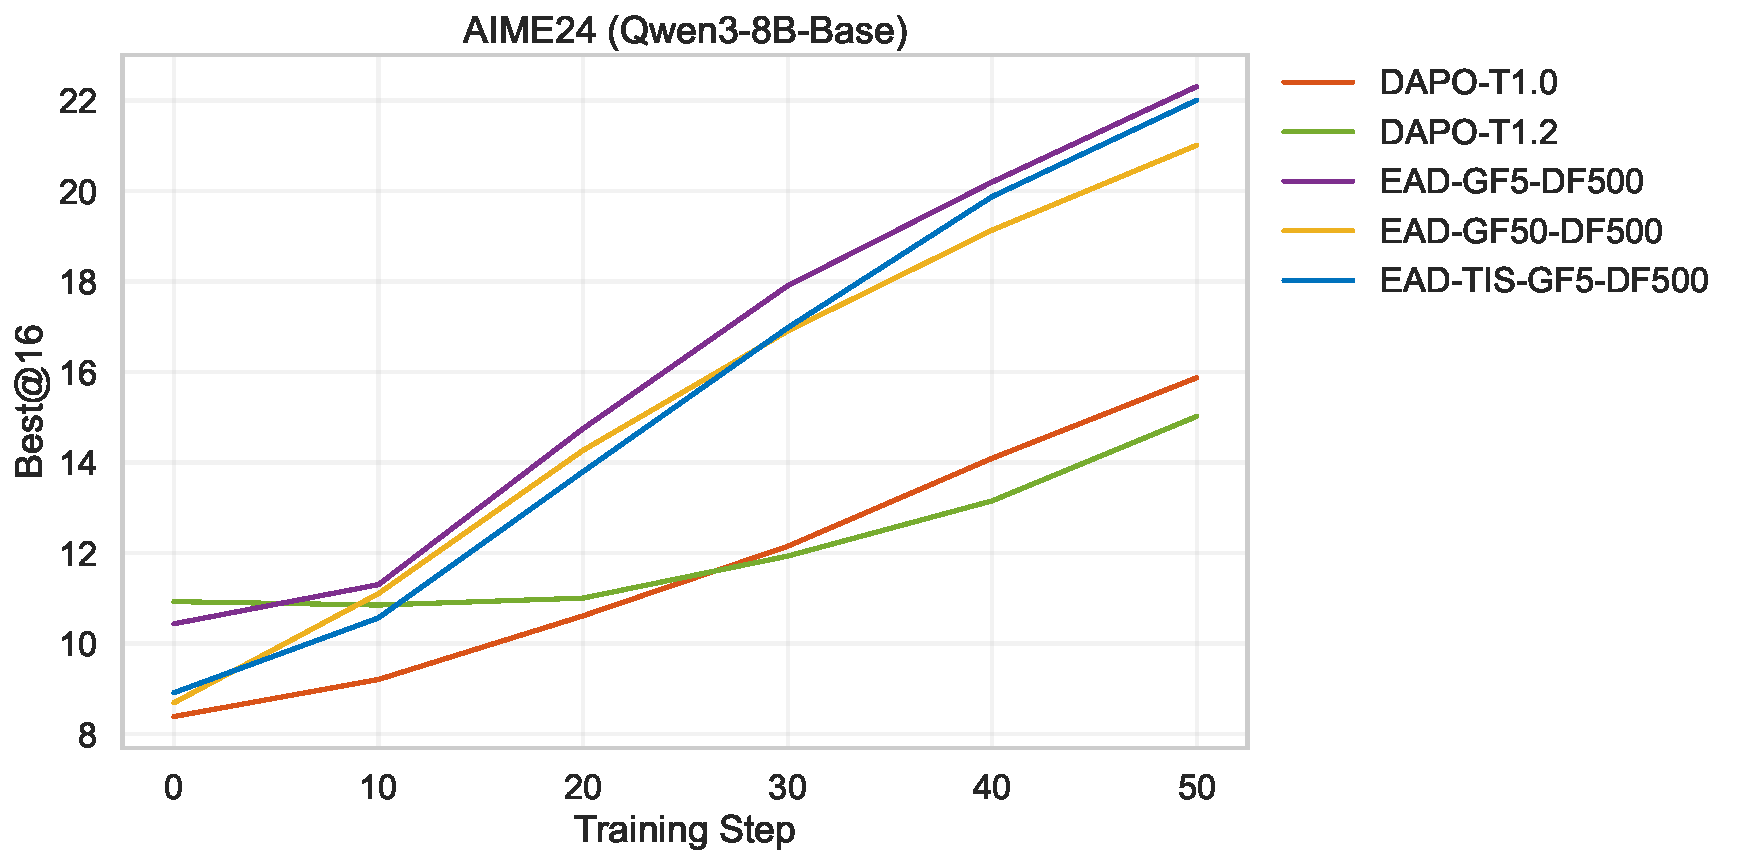
\includegraphics[width=.75\linewidth]{iclr2026/figures/stress_test_dapo16k/best_at_16_Qwen3-8B-Base.pdf}
%     \vspace{-0.1in}
%     \caption{Stress-Test \alg under DAPO recipe with challenging AIME24 benchmark as the test dataset. We can see that various setup for \alg outperforms temperature sampling baseline. } 
%     \label{fig: aime24}
%     \vspace{-0.2in}
% \end{figure}
% }
\begin{wrapfigure}{r}{0.4\textwidth}
    \centering
    \vspace{-0.85in}
    
\includegraphics[width=\linewidth]{iclr2026/figures/reverse_annealing/best_at_16_Qwen2.5-Math-1.5B-new.pdf}
    \vspace{-0.25in}
    \caption{Reverse Annealing experiment results. The reverse schedule fails to surpass normal temperature sampling.} 
    \label{fig: reverse_annealing}
    \vspace{-0.45in}
\end{wrapfigure}
\revise{
\subsection{Ablation Study}

\paragraph{Reverse Annealing} We investigate a counter-intuitive baseline where the temperature increases during generation rather than decreasing. We employ the following reverse schedule:
$\tau_t = \min\{\tau_\mathrm{min} + e^{t/d}, \tau_\mathrm{max}\}$.
We term this schedule ``RevEAD'' and report its performance in \cref{fig: reverse_annealing}. The results demonstrate that reverse annealing fails to even outperform standard temperature sampling, validating the necessity of an annealing (decreasing) temperature schedule.

\paragraph{Hyperparameter Sensitivity} 
We conduct an ablation study on the decay cap $d_{\max}$ and the growth factor $\alpha$. As shown in \cref{fig: ablation_cap}, \alg is robust to a wide range of $d_{\max}$ values, provided the cap is sufficiently large to ensure a smooth annealing schedule. Conversely, a very small cap (e.g., $d_0=d_{\max}=25$) approximates a fixed schedule (equivalent to $\alpha=0$ throughout training). This setting causes an abrupt performance drop, likely because the model cannot adapt to the increasing response lengths during training (see \cref{app: increased_length}). Alternatively, using a large initial $d_0$ yields a smooth schedule even with $\alpha=0$. However, while training remains stable, performance improves slowly due to overly conservative exploration, as shown in \cref{fig: ablation_growth_factor_and_decay_freq_init}.

% \begin{figure}[t]
%     \centering
%     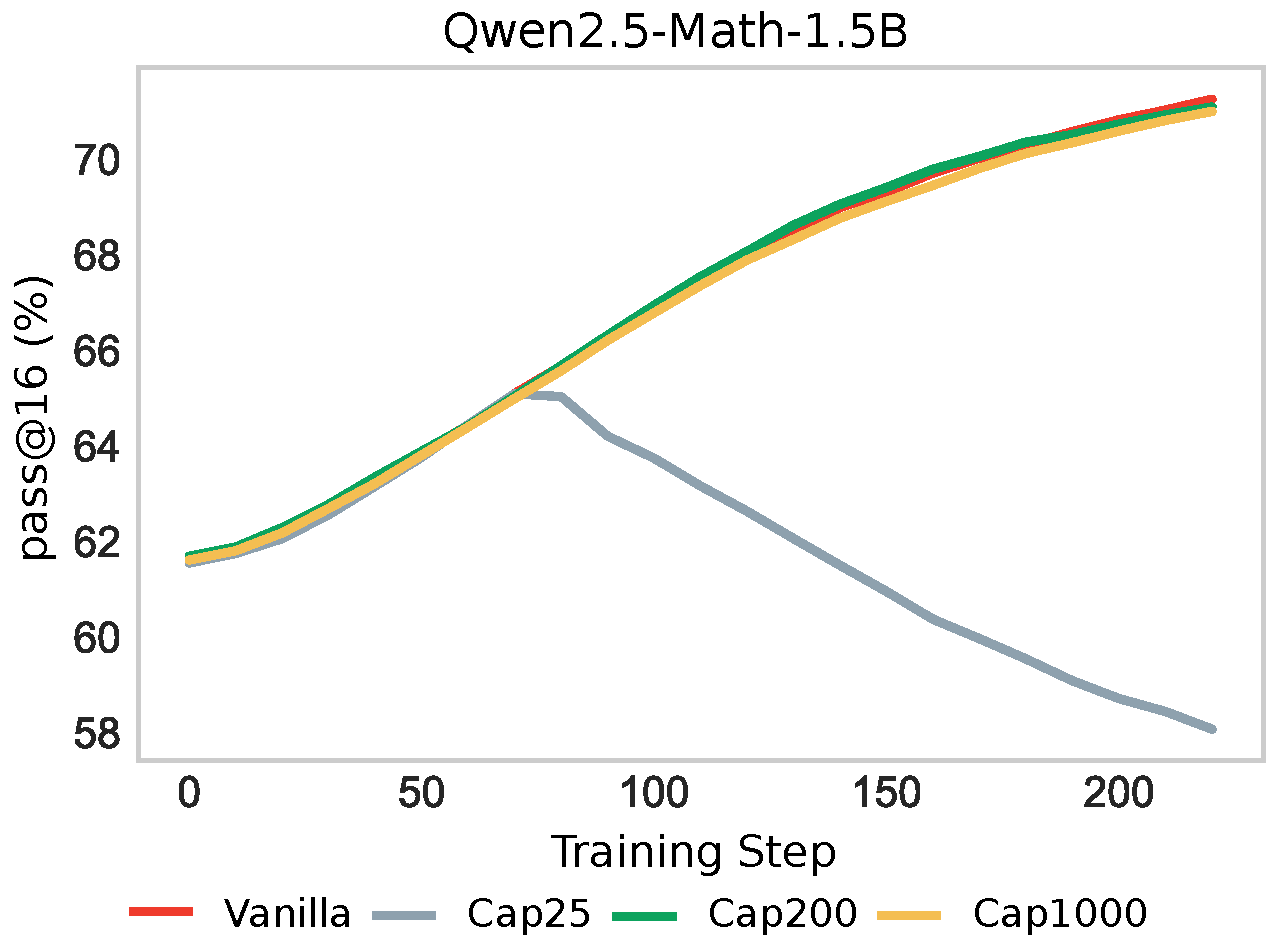
\includegraphics[width=.75\linewidth]{iclr2026/figures/ablation_cap/best_at_16_Qwen2.5-Math-1.5B-new.pdf}
%     \vspace{-0.1in}
%     \caption{Ablation on decay cap $d_{\max}$. ``\alg'' denotes the default $d_{\max}=40,000$. Setting $d_{\max}=25$ (where $d_0=25$) mimics a fixed temperature schedule (effectively $\alpha=0$), leading to performance drops as the schedule fails to adapt to longer responses. \alg remains robust provided $d_{\max}$ allows for smooth temperature reduction (e.g., $d_{\max} \ge 200$).} 
%     \label{fig: ablation_cap}
%     \vspace{-0.2in}
% \end{figure}

% \begin{figure}[t]
%     \centering
%     
\includegraphics[width=.75\linewidth]{iclr2026/figures/ablation_growth_factor_and_decay_freq_init/best_at_16_Qwen2.5-Math-1.5B-new.pdf}
%     \vspace{-0.1in}
%     \caption{Ablation on growth factor $\alpha$ and initial decay $d_0$. With a small $d_0$, a positive growth factor ($\alpha > 0$) is required to adapt to increasing response lengths and maintain a smooth intra-sequence schedule. While a large $d_0$ ensures smoothness even with $\alpha=0$, it limits exploration, resulting in lower learning efficiency.} 
%     \label{fig: ablation_growth_factor_and_decay_freq_init}
%     \vspace{-0.2in}
% \end{figure}
}

% \end{wrapfigure}

\begin{figure}[ht!]
     \centering
     \begin{subfigure}[h]{0.4\textwidth}
         \centering
         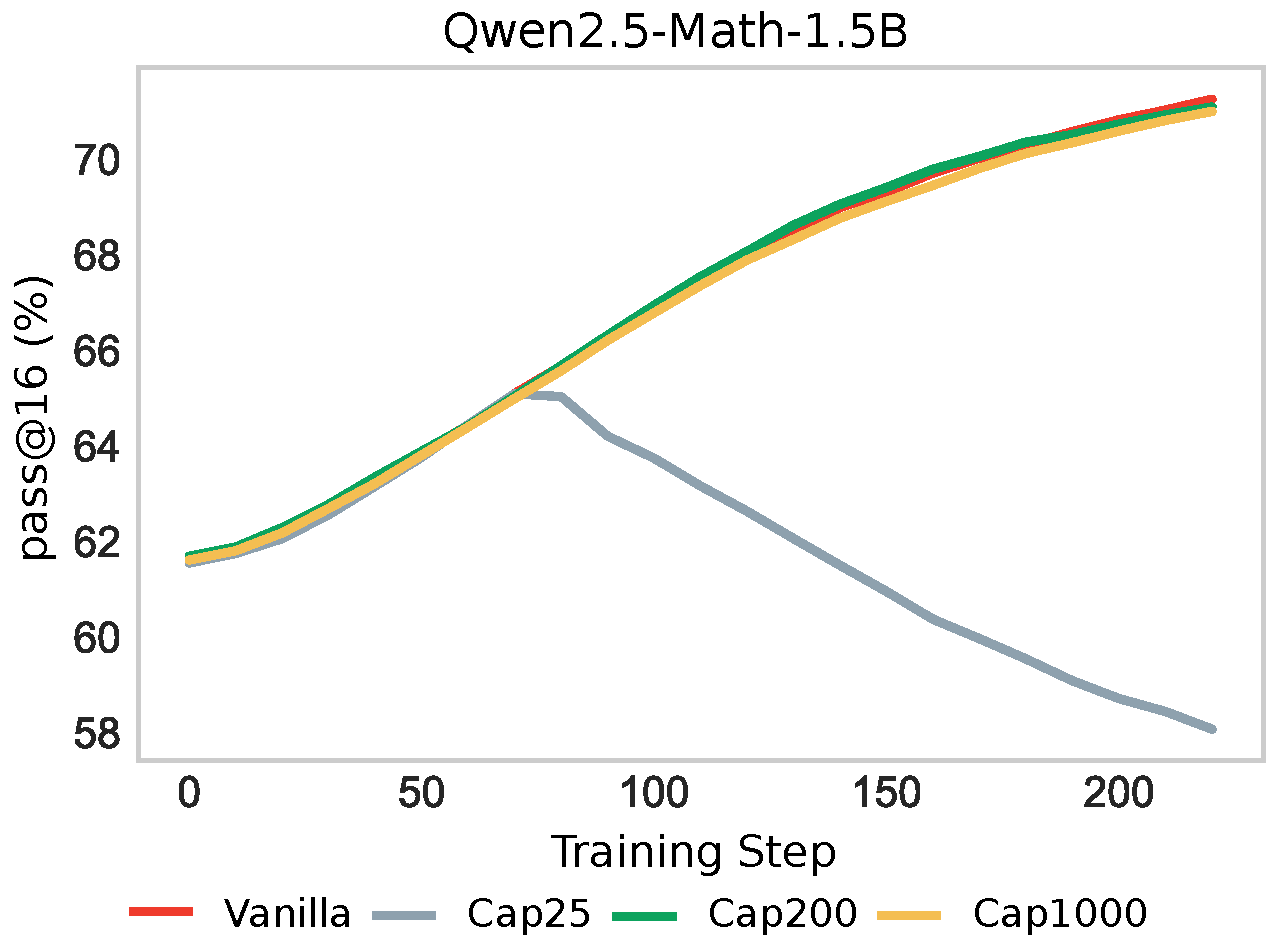
\includegraphics[width=\textwidth]{iclr2026/figures/ablation_cap/best_at_16_Qwen2.5-Math-1.5B-new.pdf}
         \caption{Decay cap $d_{\max}$.}
         \label{fig: ablation_cap}
     \end{subfigure}
     \begin{subfigure}[h]{0.39\textwidth}
         \centering
         % \vspace{-0.1in}
         
\includegraphics[width=\textwidth]{iclr2026/figures/ablation_growth_factor_and_decay_freq_init/best_at_16_Qwen2.5-Math-1.5B-new.pdf}
         \vspace{-0.2in}
         \caption{Growth factor $\alpha$ and initial decay $d_0$.}
         \label{fig: ablation_growth_factor_and_decay_freq_init}
     \end{subfigure}
\vspace{-0.1in}
\caption{Ablation on hyperparameter sensitivity. \textbf{Left:} Ablation on decay cap $d_{\max}$. ``Vanilla'' denotes EAD with the default $d_{\max}=40,000$. Setting $d_{\max}=25$ (where $d_0=25$) mimics a fixed temperature schedule (effectively $\alpha=0$), leading to performance drops as the schedule fails to adapt to longer responses. \alg remains robust provided $d_{\max}$ allows for smooth temperature reduction (e.g., $d_{\max} \ge 200$). \textbf{Right:} Ablation on growth factor $\alpha$ and initial decay $d_0$. With a small $d_0$, a positive growth factor ($\alpha > 0$) is required to adapt to increasing response lengths and maintain a smooth intra-sequence schedule. While a large $d_0$ ensures smoothness even with $\alpha=0$, it limits exploration, resulting in lower learning efficiency.}
\label{fig:hyper-parameter-sensitivity}
\vspace{-0.3in}
\end{figure}

\revise{

\subsection{Stress Test: DAPO-17K Recipe for AIME24}
To verify the effectiveness of \alg on realistic mathematical reasoning tasks, we stress-test it using the DAPO recipe~\citep{yu2025dapo}, training on DAPO-17k and evaluating on the challenging AIME 2024 benchmark. To accommodate GPU memory constraints, we utilize the Qwen-3-8B-Base~\citep{yang2025qwen3} model (instead of 32B) and reduce the maximum response length from 20,480 to 8,192. We set $d_0=500$ and $d_{\max}=40,000$, and vary $\alpha \in \{5, 50\}$. As shown in \cref{fig: aime24}, \alg achieves significant learning efficiency and consistently outperforms the standard temperature sampling baseline.

}\begin{wrapfigure}{r}{0.39\textwidth}
\vspace{-0.75in}
% \begin{figure}[t]
    \centering
    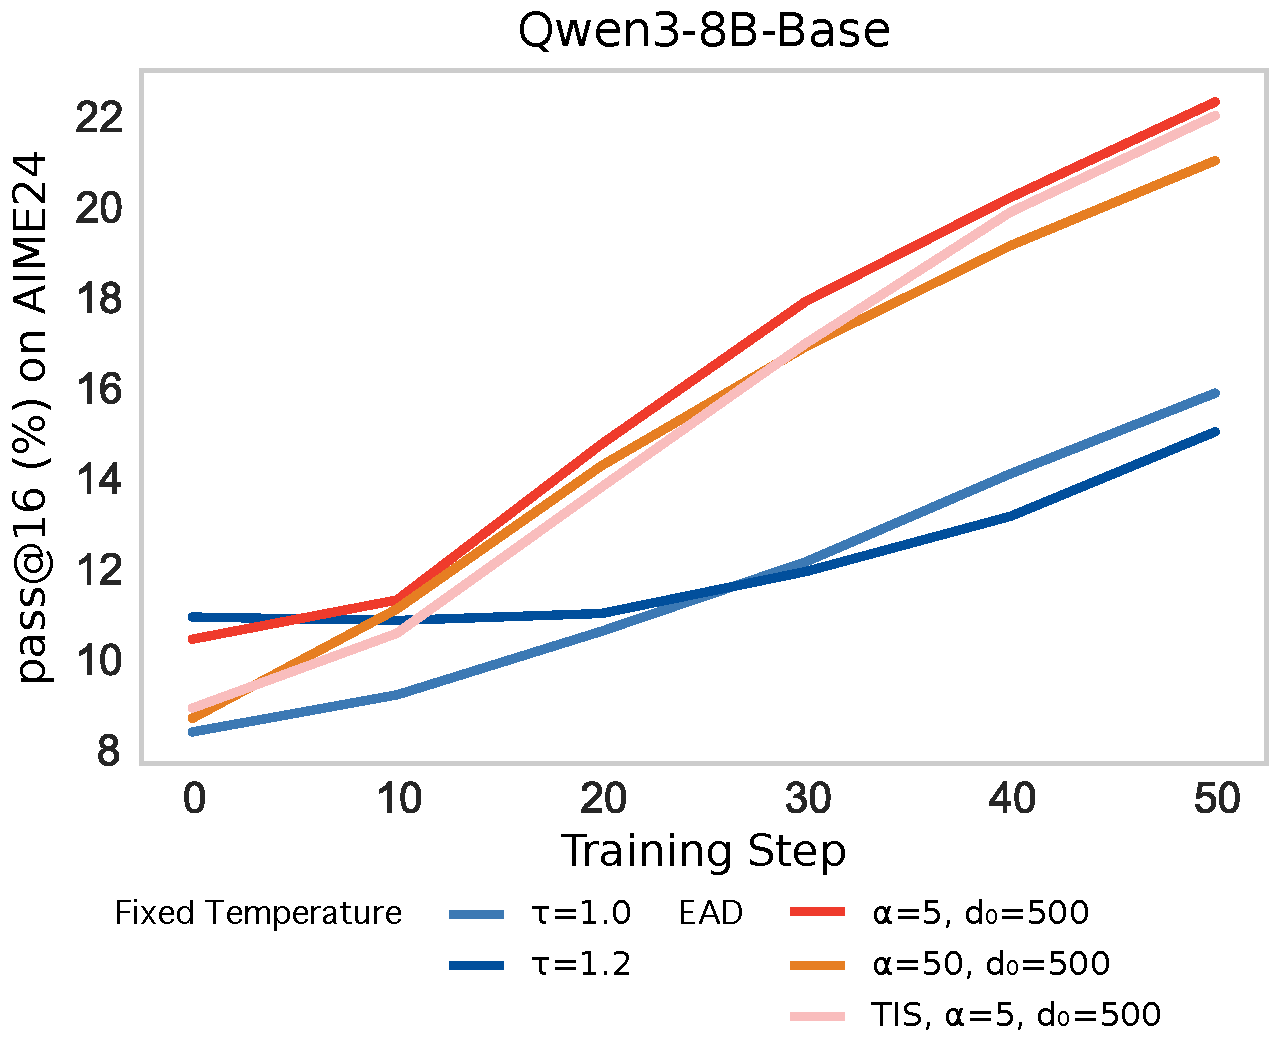
\includegraphics[width=\linewidth]{iclr2026/figures/stress_test_dapo16k/best_at_16_Qwen3-8B-Base-new.pdf}
    % \vspace{-0.2in}
    \caption{Stress-test of \alg using the DAPO recipe on AIME24. \alg outperforms the temperature sampling baseline across various hyperparameter setups.
    } 
    \label{fig: aime24}
    \vspace{-0.2in}
% \end{figure}
\end{wrapfigure}